\documentclass[11pt, a4paper]{article}

%\usepackage[T1]{fontenc}
%\usepackage{fullpage}

\usepackage[utf8]{inputenc} % comment when using lualatex
\usepackage[italian]{babel} % lingua e a-capo-sillabato
\usepackage{graphicx}
\usepackage[hidelinks]{hyperref,xcolor} % link di pagina
\usepackage[bottom]{footmisc} % note appiccicate al fondo della pagina
\usepackage{float} % per posizionamento immagini
\usepackage{amsthm}
\usepackage{fancyhdr}
\usepackage[font=small,labelfont=bf]{caption} % small font for caption (and bold Figure word)
\usepackage{fontawesome} % for github icons

\pagestyle{fancy}
\fancyhf{}% Clear header/footer
\fancyfoot[C]{\thepage} %add page number
\fancyhead[C]{\footnotesize\textit{Documento:} D4 \hfill SleepCode \hfill \textit{Versione:} 1.0}
\renewcommand{\headrule}{{\color{red!70}\rule{\textwidth}{2pt}}}
\setlength{\headheight}{22pt}
\hypersetup{
    colorlinks=true,
    linkcolor=black,
    filecolor=magenta,      
    urlcolor=blue,
    }

%\pagestyle{myheadings}
%\markright{John Smith\hfill On page styles\hfill}

\renewcommand\UrlFont{\color{blue}\rmfamily}

\theoremstyle{definition}

\newtheorem{funcreq}{RF} %% numerazione dei requisiti funzionali
\newtheorem{nonfuncreq}{RNF} %% requisiti non funzionali
\newtheorem{backend}{BE}
\newtheorem{frontend}{FE}

\title{Documento di Sviluppo}

\author{Raffaele \textsc{Castagna}\\
Alberto \textsc{Rovesti}\\
Zeno \textsc{Saletti}}

\newcommand{\groupNumber}{G17}


% —

% Web address for the project (if any)
% \newcommand{\homepage}{\url{https://www.}}

% data
\date{\today}

\makeatletter{}


\newcommand\blfootnote[1]{%
  \begingroup
  \renewcommand\thefootnote{}\footnote{#1}%
  \addtocounter{footnote}{-1}%
  \endgroup
}

% IL PREAMBOLO FINISCE QUI %%%%%%%%%%%%%%%%%%%%%%%%%%%%%%%%%%%%%%%%%%%%%%%%%%%%






\begin{document}

% La pagina di copertina si trova in un file .tex a parte
% NON MODIFICARE QUESTO COMANDO!!!
\begin{titlepage}
\newcommand{\HRule}{\rule{\linewidth}{0.3mm}} % Defines a new command for horizontal lines, change thickness here
\center % Centre everything on the page

%------------------------------------------------
%	Logo
%------------------------------------------------

\includegraphics[width=0.3\textwidth]{materiale/UniTrento_logo_ITA_colore.png}\\[0.5cm]
%------------------------------------------------
%	Headings
%------------------------------------------------
\textsc{\Large Dipartimento di Ingegneria\\e Scienza dell'Informazione}\\[1.5cm]

{\Huge\textbf{Sleep Code}}\\[0.5cm]
\textsc{\large Progetto per il Corso di Ingegneria del Software}\\
\textsc{\large Anno Accademico 2023-2024}\\[0.5cm]

%------------------------------------------------
%	Title
%------------------------------------------------

\HRule\\[0.4cm]
{\huge\bfseries \@title}\\[0.1cm]
\HRule\\[1cm]

\begin{minipage}{\textwidth}
\begin{flushleft}
\textit{Descrizione:} documento di analisi dei requisiti funzionali, non funzionali, front-end e back-end.
\end{flushleft}
\end{minipage}\\[1.5cm]


\begin{minipage}{0.4\textwidth}
\begin{flushleft}
\large
\textit{Numero documento:} D1
\end{flushleft}
\end{minipage}
\begin{minipage}{0.4\textwidth}
\begin{flushright}
\large
\textit{Versione documento:} 2.4
\end{flushright}
\end{minipage}\\[1.5cm]

%------------------------------------------------
%	Author(s)
%------------------------------------------------
\begin{minipage}{0.4\textwidth}
\begin{flushleft}
\large
\textit{Membri del gruppo:}\\
\@author % Your name
\end{flushleft}
\end{minipage}
~
\begin{minipage}{0.4\textwidth}
\begin{flushright}
\large
\textit{Numero gruppo: }
\groupNumber
\end{flushright}
\end{minipage}

% 	If you don't want a supervisor, uncomment the two lines below and comment the code above
% 	{\large\textit{Author(s)}}\\
% 	\@author % Your name

%------------------------------------------------
%	Date
%------------------------------------------------

\vfill\vfill
\textit{Ultima revisione:}
{\@date}

\end{titlepage}

\tableofcontents\blfootnote{\textbf{Consigli utili per la consultazione del testo:} Se il lettore per file \texttt{.pdf} attualmente in uso lo consente, è possible navigare con più semplicità e velocità all'interno di questo documento cliccando sugli elementi dell'indice.}


\newpage
\section{Scopo del documento}
Il presente documento riporta tutte le informazioni richieste e necessarie per lo Sviluppo
di una parte dell'applicazione Sleepcode.
In particolare, presenta:
\begin{itemize}
  \item User Flow legato al ruolo dell'utente (amministratore,autenticato e non)
  \item User Flow legato all'uso del sito
  \item Documentazione delle Api attraverso API Model e Modello delle risorse
  \item Api Fornite per interagire con l'applicazione
  \item Descrizione delle api fornite
  \item Risultati delle test suite applicata sulle api
\end{itemize}


\newpage
\section{User Flows}
In questa sezione del documento di sviluppo vengono riportati gli User Flows. Lo scopo degli User Flows
è quello di poter specificare le azioni disponibili all'utente e le conseguenza di esse. Sono stati individuati 2 tipi di User flow, uno per 
tutto ciò che riguarda l'autenticazione e il profilo utente, e un'altro che riguarda le azioni disponibili ai diversi ruoli di utente.
Teniamo a ricordare che tutte le immagini sono disponibili ad alta risoluzione nell'appropriata cartella del D4.
Di seguito esponiamo la legenda per i simboli utilizzati
\\
\\
\begin{center}
  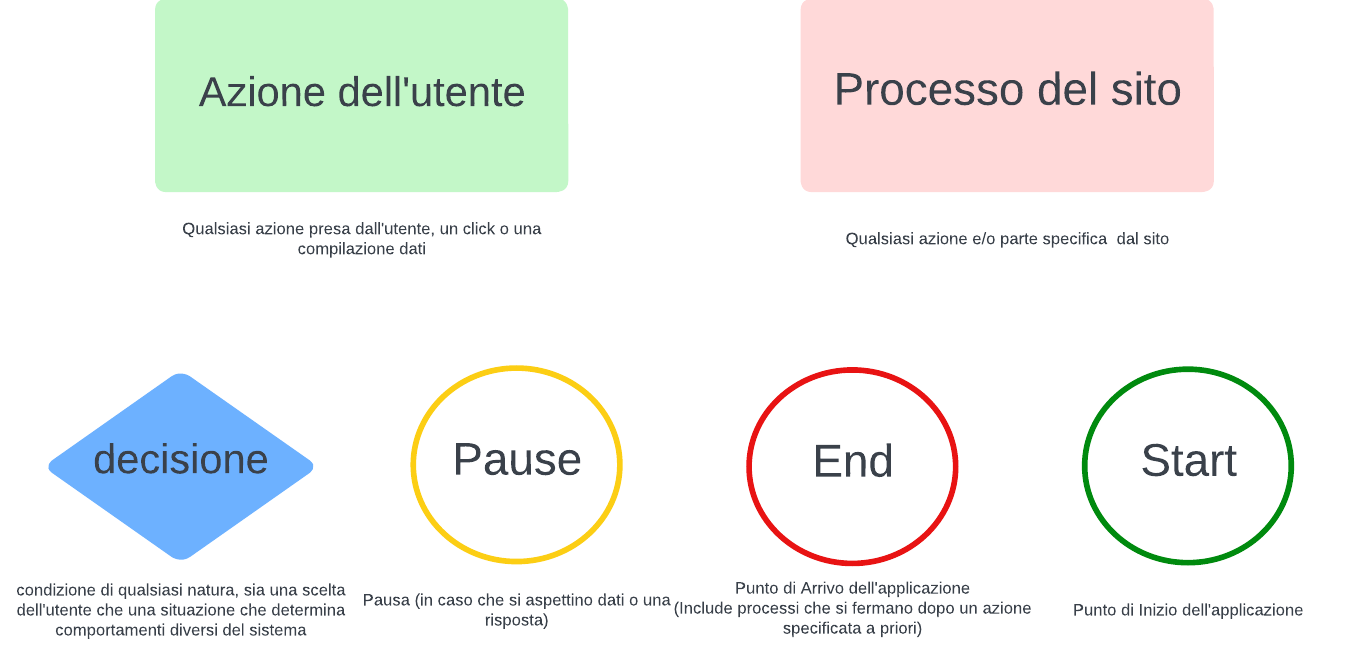
\includegraphics{materiale/UserFlow Symbols.png}
\end{center}
\newpage
\subsection{Azioni riguardanti l'autenticazione}
Questo User Flow è specifico per tutte le azioni che riguardo l'autenticazion e ciò che fa parte di essa. Si ricorda che in ogni momento della navigazione
l'utente è in grado di poter autenticarsi,tornare alla home e al catalogo tramite una apposita Navbar che è presente in ogni pagina del sito web. Parte di queste interazioni sono state rimosse per
rendere l'User Flow pià leggibile.
  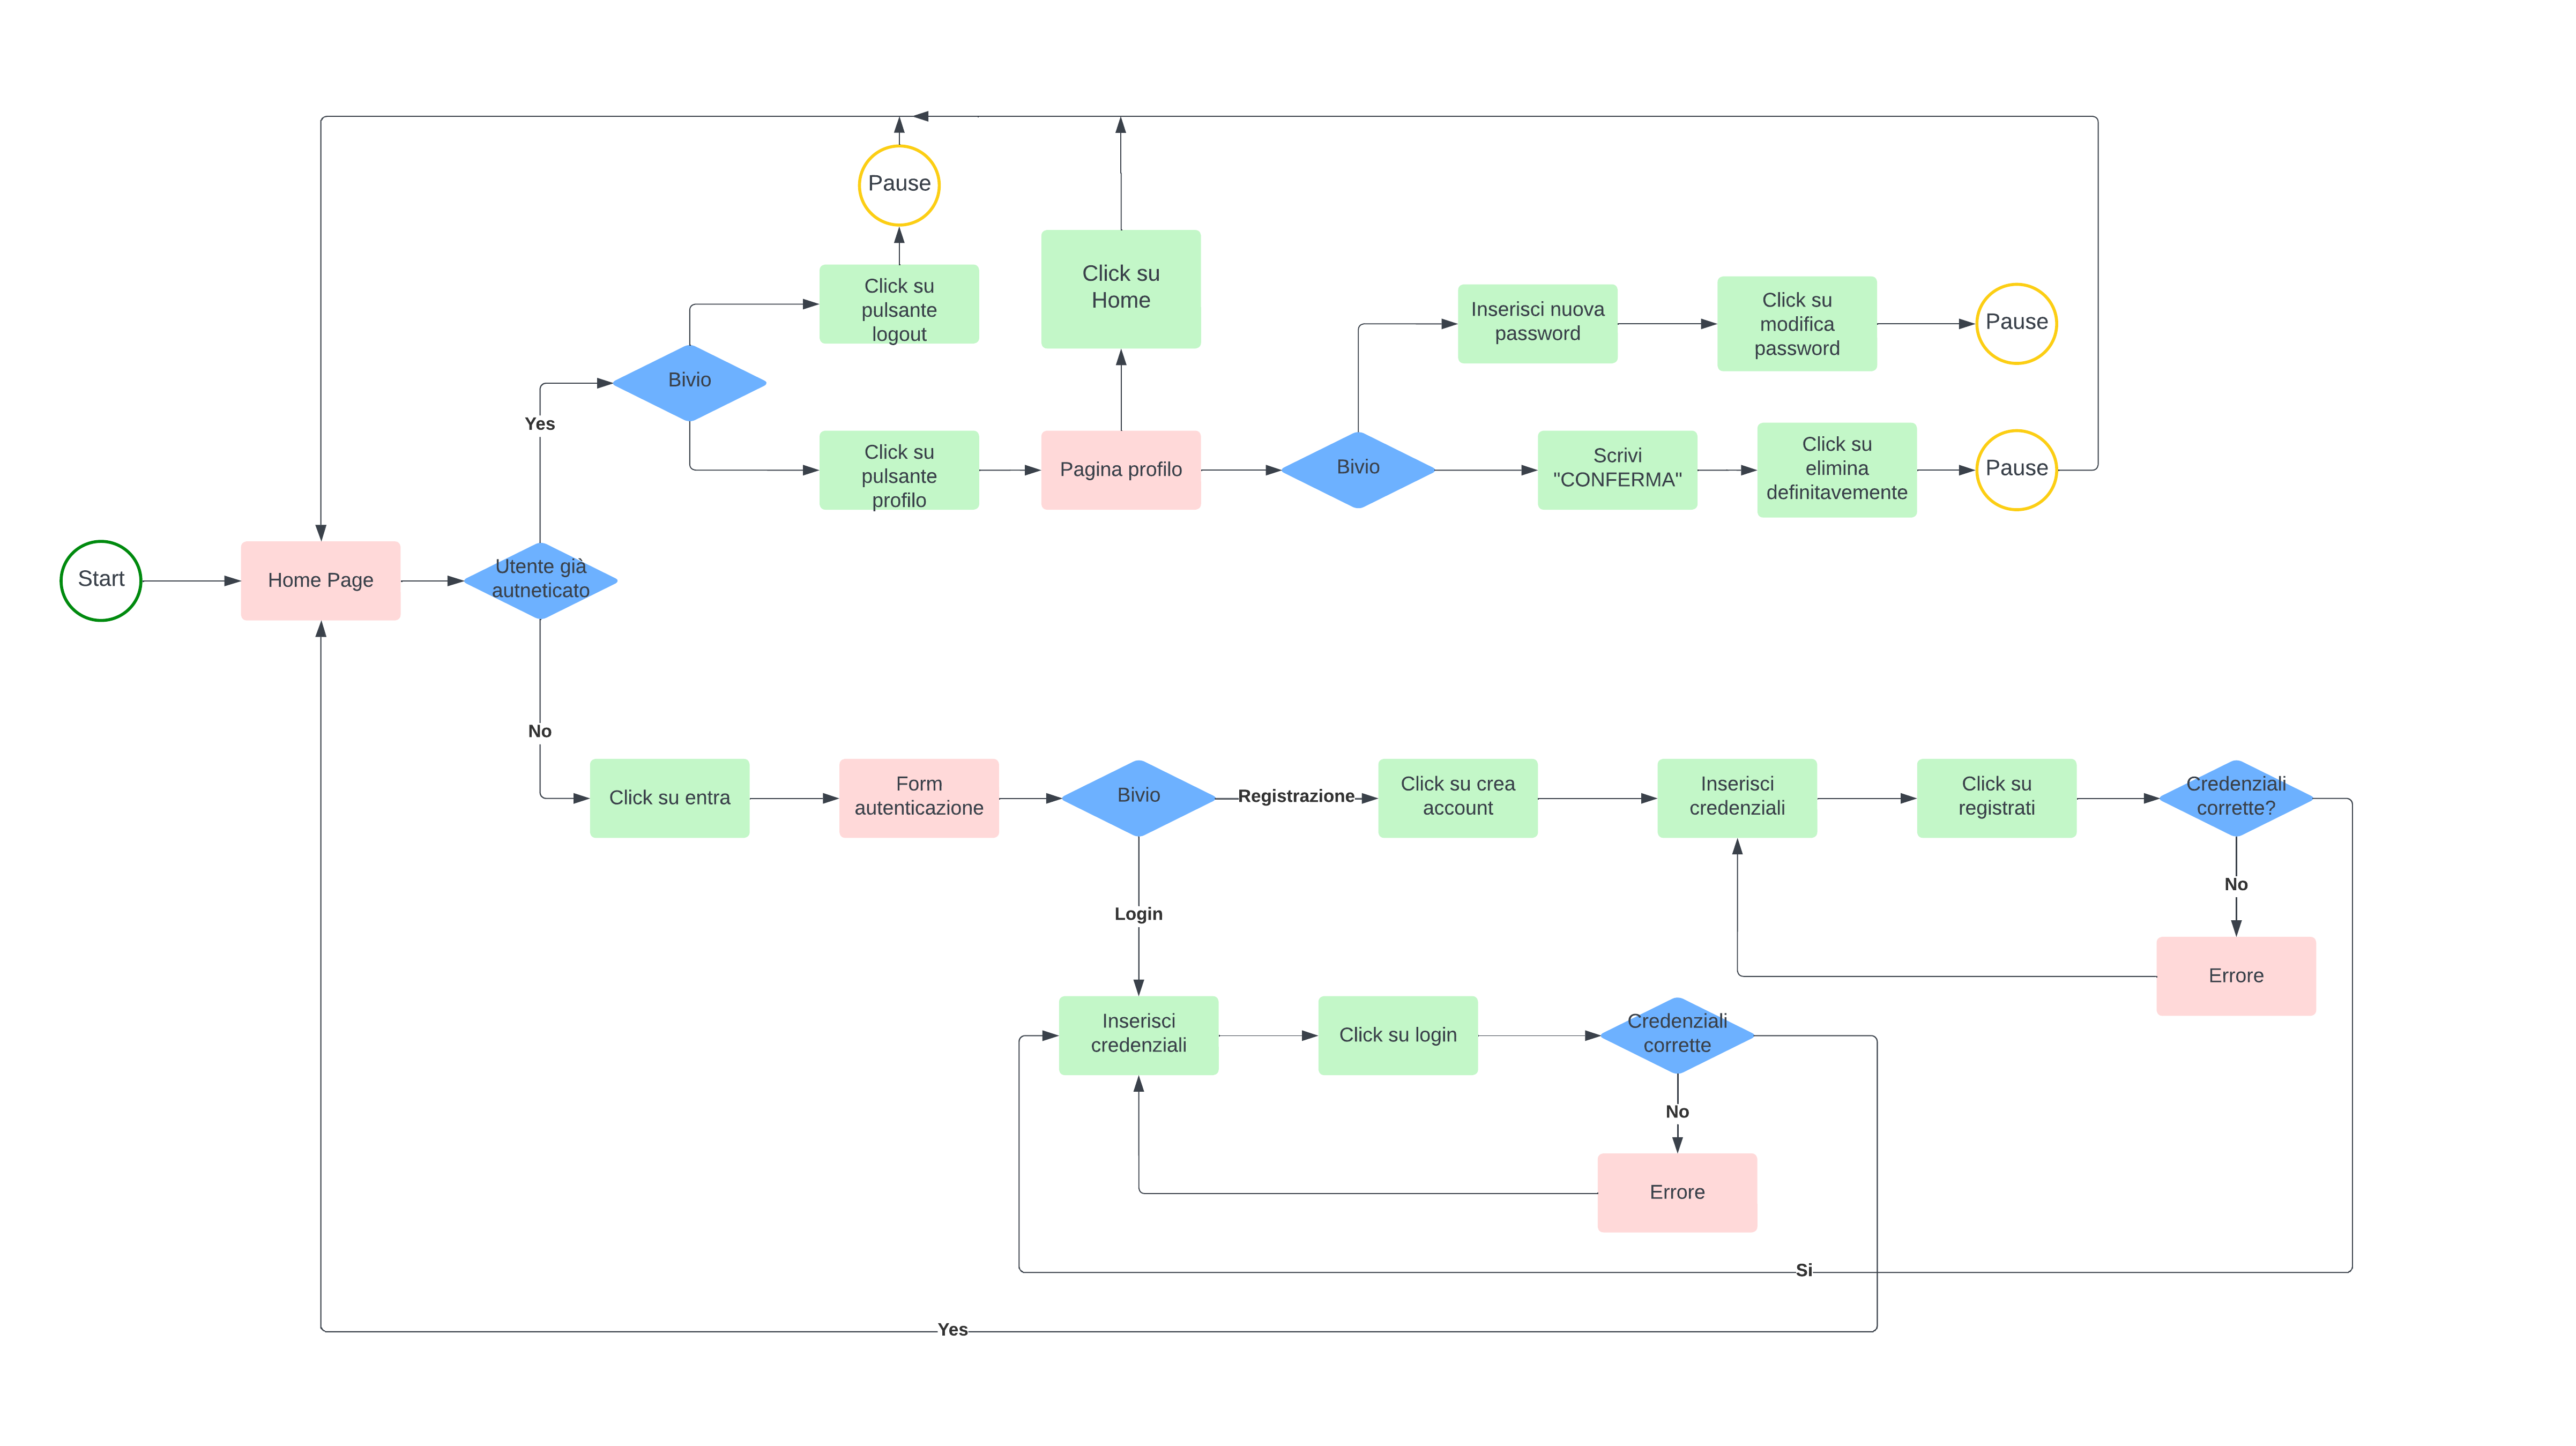
\includegraphics[width=\textwidth]{materiale/UserFlow Autenticazione.png}
\newpage
\subsection{Azioni riguardanti l'utilizzo del sito}
Questo User Flow è specifico per tutte le azioni che ogni tipo di utente può intraprendere nell'utilizzo del sito, teniamo a precisare che la funzione di aggiunta di un problema tramite DB non è stata sviluppata, al momento il form esiste
ma non dialoga col database, ci scusiamo per l'incovenienza. Ricordiamo che tramite Navbar l'utente è in grado di intraprendere tutte le azioni descritte nell'User Flow precedente.

  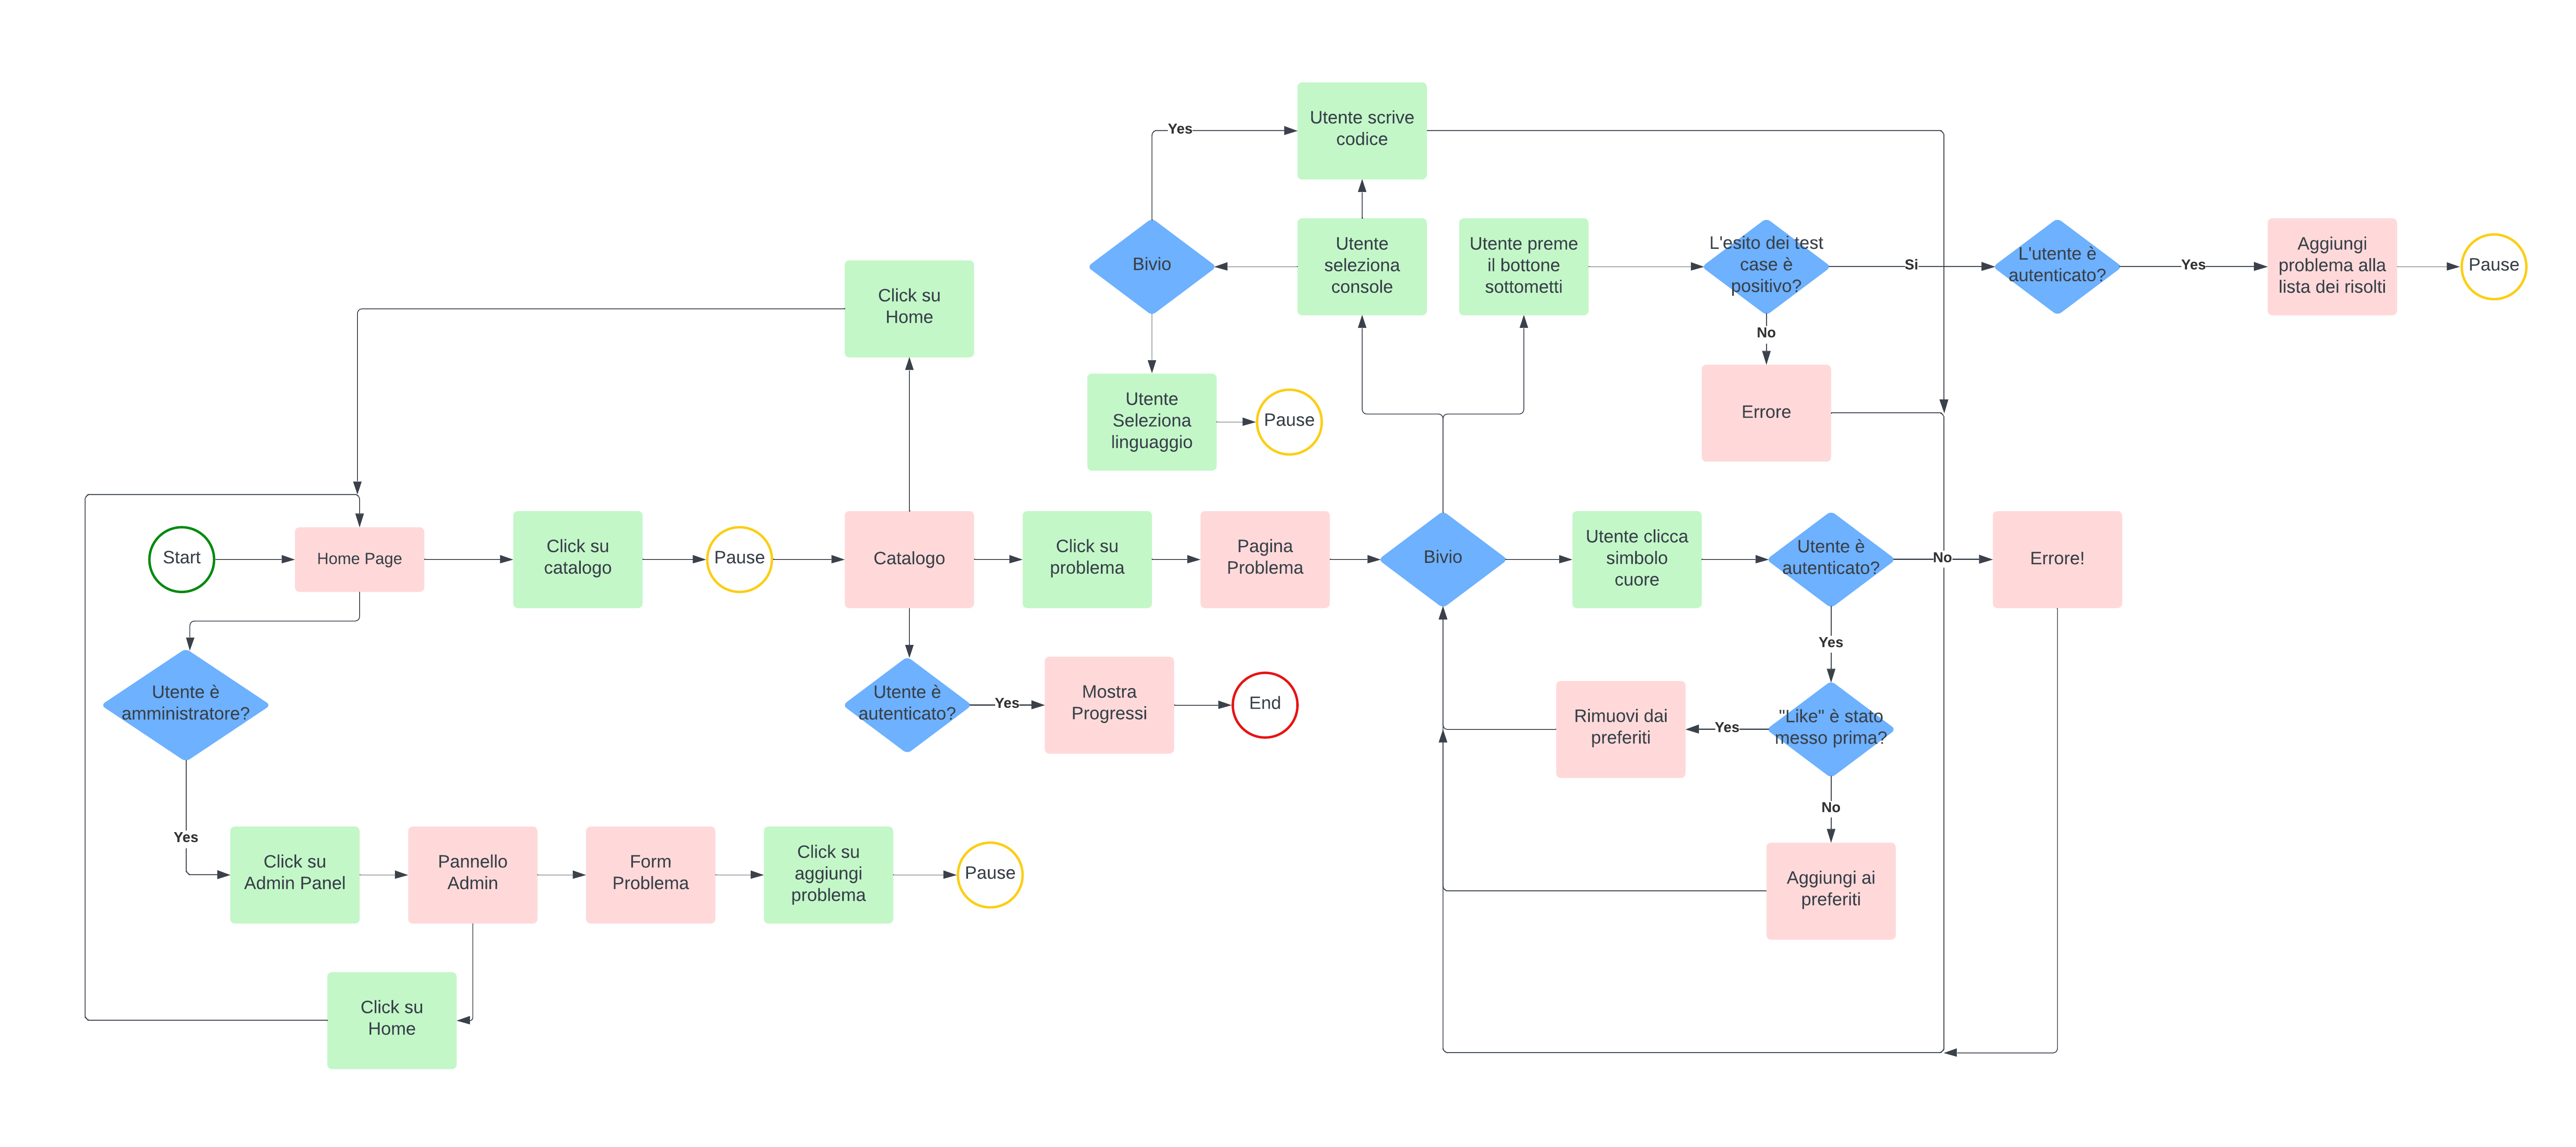
\includegraphics[width=\textwidth]{materiale/UserFlow Utilizzo.png}

\newpage
\section{Documentazione e implementazione dell'applicazione}
Nella precedente sezione abbiamo illustrato tutte le funzioni attualmente implementate nell'applicazione e un'idea di come l'utente può interagire con esse.
L'applicazione \textbf{SleepCode} è stata sviluppata utilizzando \href{https://nextjs.org/}{Next.js} vers. 14.0.3, un framework Javascript free-open source basato su \href{https://react.dev/}{React}

\subsection{Struttura del Progetto}
Il software utilizzato per version control utilizzato è \href{https://git-scm.com/}{Git}, come remote repository abbiamo utilizzato \href{www.github.com}{Github},
il codice e la sua history è presente su una repository del membro del Team Raffaele Castagna, l'ultima versione stabile e quella utilizzata per hostare il sito è disponibile presso la repository CodeBase, all'interno di essa,
troveremo le seguenti cartelle:
\\
\begin{center}
  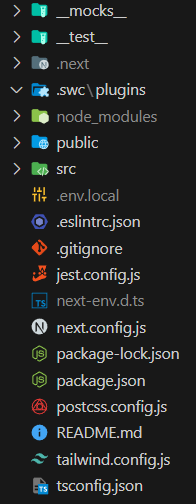
\includegraphics{materiale/Project Structure.png}
\end{center}
Ricordiamo che le cartelle \textbf{.next, .swc, .env} insieme a \textbf{package-lock.json, next-env.d.ts, eslintrc.json} sono state generate automaticamente
\newpage
\subsubsection{Directory: \_\_mock\_\_ }
Questa cartella contine delle funzioni "mock" che permettono a Jest di poter effetuare il testing senza fare chiamate dirette al database.
\subsubsection{Directory: \_\_test\_\_}
Questa cartella contiene tutti i test case e test suite dedicate al testing.
\subsubsection{Directory: public}
Questa cartella contiente tutte le immagini utilizzate all'interno del sito.
\subsubsection{Directory: src}
Questa cartella contiente tutte le parti del progetto sia front-end che back-end del progetto, procediamo con una vista più dettagliata
\begin{center}
  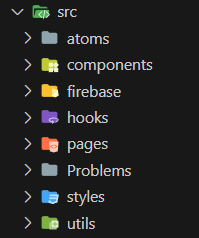
\includegraphics{materiale/src.png}
\end{center}
\begin{itemize}
  \item \textbf{Atoms}: Abbiamo utilizzato una libreria di State management sviluppata da Google per tenere traccia dello stato dell'utente, la libreria utilizzata è: \href{https://recoiljs.org/}{Recoil}, gli atoms non sono altro che gli stati di certi componenti del sito.
  \item \textbf{Components}: Questa cartella contiene tutti i vari componenti del sito che vengono utilizzati dalle pagine, essi possono essere semplici \href{https://www.nngroup.com/articles/skeleton-screens/}{Scheletri} o componenti di maggior importanza.
  \item \textbf{Firebase}: Questa cartella contiene tutti i file relativi al setup di \href{https://firebase.google.com/}{Firebase}, il database utilizzato per il progetto.
  \item \textbf{Hooks}: Questa cartella contiene gli hooks sviluppati durante il progetto per compiere una funzione.
  \item \textbf{Pages}: Questa Cartella contiente le varie pagine le loro \textbf{routes} e le \textbf{API}.
  \item \textbf{Problems}: Questa cartella contiene il tipo di dato generico per i problemi.
  \item \textbf{Styles}: Questa cartella contiene diversi stili pre-impostati utilizzati assieme a \href{https://tailwindcss.com/}{TailwindCSS}
  \item \textbf{Utils}: Questa cartella contiene i diversi testi e informazioni relative ai problemi attualmente disponibili, oltre che a form validators e funzioni comuni.
\end{itemize}
\subsubsection{.env.local}
Questa file contiene tutte le \textbf{variabili locali}, utilizzate per la connessione al database e necessarie per il corretto funzionamento dell'applicativo.
\subsubsection{.gitignore}
Questa cartella specifica quali file \textbf{git} non deve includere nelle varie pull/push requests. (.env.local è la più importante in quanto contiente la \textbf{Chiave segreta})
\subsubsection{jest.config.js}
Questo file contiene la configurazione di \textbf{Jest}, libreria utilizzata nel testing.
\subsubsection{package.json}
Questo file contiene le \textbf{dependency} del framework
\subsubsection{README.md}
Questo file contiene informazioni generali sul progetto.
\subsubsection{postcss.config.js}
Questo file è stato auto-generato da \href{https://tailwindcss.com/}{TailwindCSS}
\subsubsection{tailwind.config.js}
Questo file contiene \textbf{pallet} di colori utilizzati da \href{https://tailwindcss.com/}{TailwindCSS}
\subsubsection{tsconfig.json}
Questo file contiene regole utilizzate da \href{https://eslint.org/}{ESLint} un \textbf{patter checker} utilizzato durante lo sviluppo
  
\subsection{Dependencies del progetto}
Il progetto utilizza diverse librerie, procediamo ad elencarne le più importanti e spiegare il loro funzionamento.
\begin{itemize}
  \item \href{https://codemirror.net/}{\textbf{CodeMirror}}: Utilizzata nel front-end avere uno stile simile a Vs-code durante la scrittura del codice.
  \item \href{https://split.js.org/}{\textbf{Split}}: Utilizzata nel front-end per rendere la pagina dei problemi dinamica (L'utente è in grado di modificare la grandezza dei componenti).
  \item \href{https://www.npmjs.com/package/react-toastify}{\textbf{Toastify}}: Libreria che offre componenti UI utilizzati per dialogare con l'utente.
  \item \href{https://recoiljs.org/}{\textbf{Recoil}}: Libreria di State Management sviluppata da Google.
  \item \href{https://firebase.google.com/docs/build}{\textbf{Librerie fornite da Firebase}}: Abbiamo utilizzato diverse librerie fornite da firebase come \textbf{auth,sdk,admin sdk} e molte altre.
  \item \href{https://www.npmjs.com/package/yup}{\textbf{Yup}}: Utilizzato per la validazione RegEx di dati inseriti
  \item \href{https://eslint.org/}{\textbf{ESLint}}: Pattern checker utilizzato durante lo sviluppo per ottenere un codice di alta qualità
  \item \href{https://jestjs.io/}{\textbf{Jest}}: Libreria utilizzata per il testing
  \item \href{https://www.npmjs.com/package/node-mocks-http}{\textbf{node-mocks-http}}: Libreria utilizzata per mandare richieste API finte durante il testing.
\end{itemize}
Oltre a queste abbia altre dipendenze minore tra vari \textbf{hooks} e pacchetti necessari per altri pacchetti inutili da elencare.
\subsection{Dati del Progetti e Database}
Per il corretto funzionamento del sito, l'applicazione necessità della consultazione di alcuni file locali, in seguito elencheremo alcune strutture dati utilizzate.
\subsubsection{Database}
Il database scelto per memorizzare i dati è \href{https://firebase.google.com}{\textbf{Firebase}},per essere più specifici \textbf{Firestore}, il sottoinsieme che si occupa della memorizazzione dei dati in cloud.
Sono state individuate due collezioni da dover inserire nel database e due collezioni da tenere in locale per facilitare lo sviluppo così da poter operare in maniera 'strict'
\newpage
\textbullet   \textbf{ Problem}\\
Questo modello rappresenta un Problema Generico all'interno dell'applicazione, ciò che l'applicazione sa su un problema è differente da ciò che il database tiene memorizzato, questo sia per motivi di facilità che limiti sui dati che possiamo tenere nel cloud.
Ci sono alcuni campi la quale funzione non è immediatiamente chiara, quindi elencheremo la funzione di ogni campo.
\begin{itemize}
  \item \textbf{id}: l'id del problema, per semplicità l'id dei problemi è il loro titolo in minuscolo con "-" al posto degli spazi.
  \item \textbf{title}: Il nome del problema.
  \item \textbf{problemStatement}: La descrizione del problema.
  \item \textbf{examples}: Contiente tutti gli esempi che vogliamo mostrare all'utente.
  \item \textbf{constraints}: Nel caso gli input e/o output abbiano certe regole da rispettare questa campo le conterrà.
  \item \textbf{order}: Ad ogni problema assegneremo un numero che verrà utilizzato nell'ordinamento dei problema nella pagina principale.
  \item \textbf{starterCode}: Le linee di testo presenti appena si apre un problema per la prima volta
  \item \textbf{handlerFunction}: Funzione associata ad ogni problema che permette la sottomissione e il controllo del codice scritto dall'utente.
  \item \textbf{starterFunctionName}: Nome della funzione associata al problema.
\end{itemize}

\begin{center}
  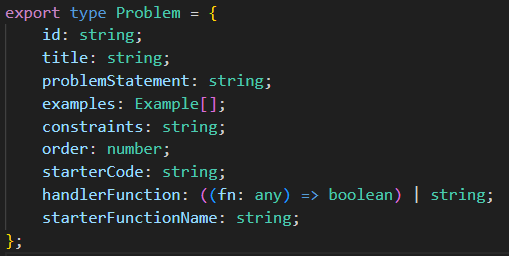
\includegraphics[width=10cm]{materiale/Problem Template.png}
\end{center}
\newpage
\textbullet   \textbf{ Example}\\
Questo modello rappresenta come deve essere strutturato un esempio all'interno del problem. Include due campi opzionali (\textbf{explanation,img}) che possono non essere presenti su alcuni problemi.

\begin{center}
  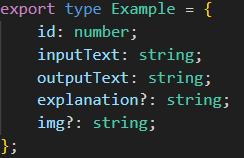
\includegraphics[width=5cm]{materiale/Example Template.png}
\end{center}

\newpage
\textbullet   \textbf{ DBProblem}\\
Questo modello rappresenta i dati che vengono raccolti dal database riguardanti ogni problema, anche qui abbiamo un campo opzionale \textbf{videoId}.
\begin{center}
  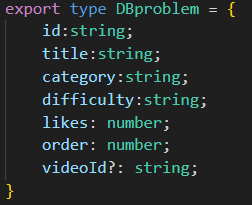
\includegraphics[width=5cm]{materiale/DBProblem Template.png}
\end{center}
\newpage
\textbullet \textbf{ userData}
Questo Modello rappresenta i dati che riguardano ogni utente al momento della registrazione, il ruolo di "\textbf{User}" viene assegnato inizialmente ad ogni utente e successivamente attraverso console di Firestore verrà cambiato manualmente a "\textbf{Administrator}"
se si vuole promuovere l'utente.
\begin{center}
  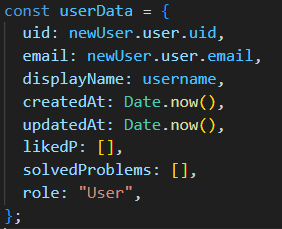
\includegraphics[width=5cm]{materiale/User Template.png}
\end{center}
\newpage
\subsection{Project API}
In questa parte del documento presentiamo le API dell'applicazione Sleepcode.
Le descriveremo prima e successivamente mostreremo il loro codice.
\subsubsection{Estrazione delle risorse dal class diagram}
Analizzando il diagramma delle classi abbiamo individuato due risorse principali: l'utente e i problemi, di seguito riportiamo le api:
\subsubsection{API riguardanti l'utente}
\begin{itemize}
  \item \textbf{signup (POST)}: Questa API permette all'utente non ancora autenticato di creare un account sulla nostra piattaforma per tracciare i progressi. Se tutte le informazioni sono valide l'account verrà create altrimenti l'utente riceverà un errorre.
  \item \textbf{deleteaccount (DELETE)}: Questa API permette all'utente autenticato di eliminare il proprio account e tutte le informazioni associate ad esso. (I "like" lasciati dall'utente rimarrano nel Database in modo da avere uno storico dei problemi più accurato)
  \item \textbf{changepassword (PATCH)}: Questa API permetet all'utente autenticato di poter cambiare la propria password dal sito stesso. Se le informazioni sono valide la password verrà cambiata altrimenti l'utente riceverà un errore.
\end{itemize}

\subsubsection{API riguardanti i problemi}
\begin{itemize}
  \item \textbf{getProblems (GET)}: Questa API viene chiamata quando un utente (autenticato o no) si connette alla pagina del catalogo, essa ritorna la lista di problemi disponibili in quel momento.
\end{itemize}
\newpage
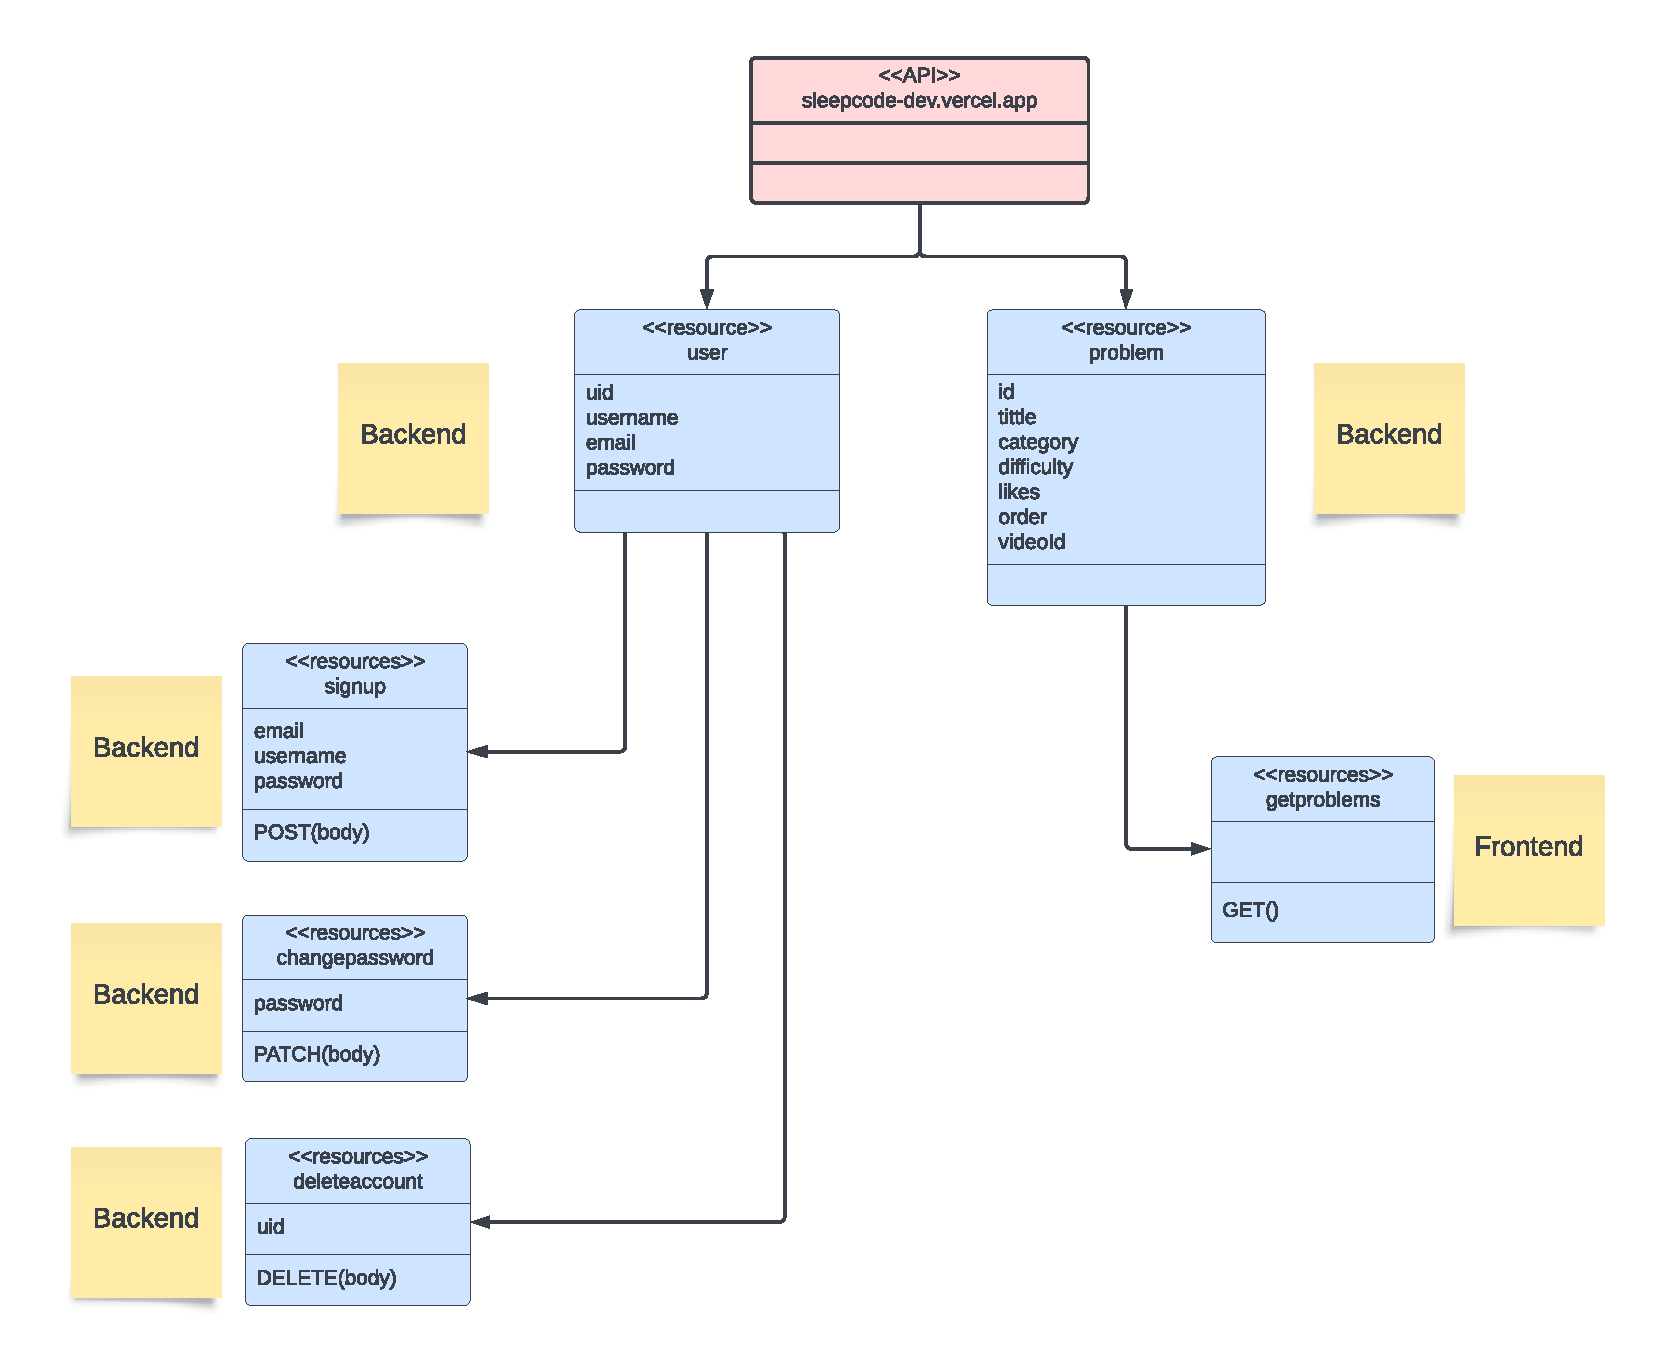
\includegraphics[width=\textwidth]{materiale/Resource diagram.png}
\subsubsection{Resource Models}
Il Resource model esprime, per ogni API, le diverse risposte, come sono strutturate le richiesta e come ci si può accedere.
Ogni API dovrà elaborare il body (se lo richiede), ovvero le informazioni necessarie per il corretto funzionamento, e risponderà appropriatamente con uno \href{https://developer.mozilla.org/en-US/docs/Web/HTTP/Status}{Status Code}.
Il body viene rappresentato tramite una freccia che entra e le risposte sono rappresentate tramite delle freccie che escono.\\
\newpage
\textbullet \textbf{ User API}\\
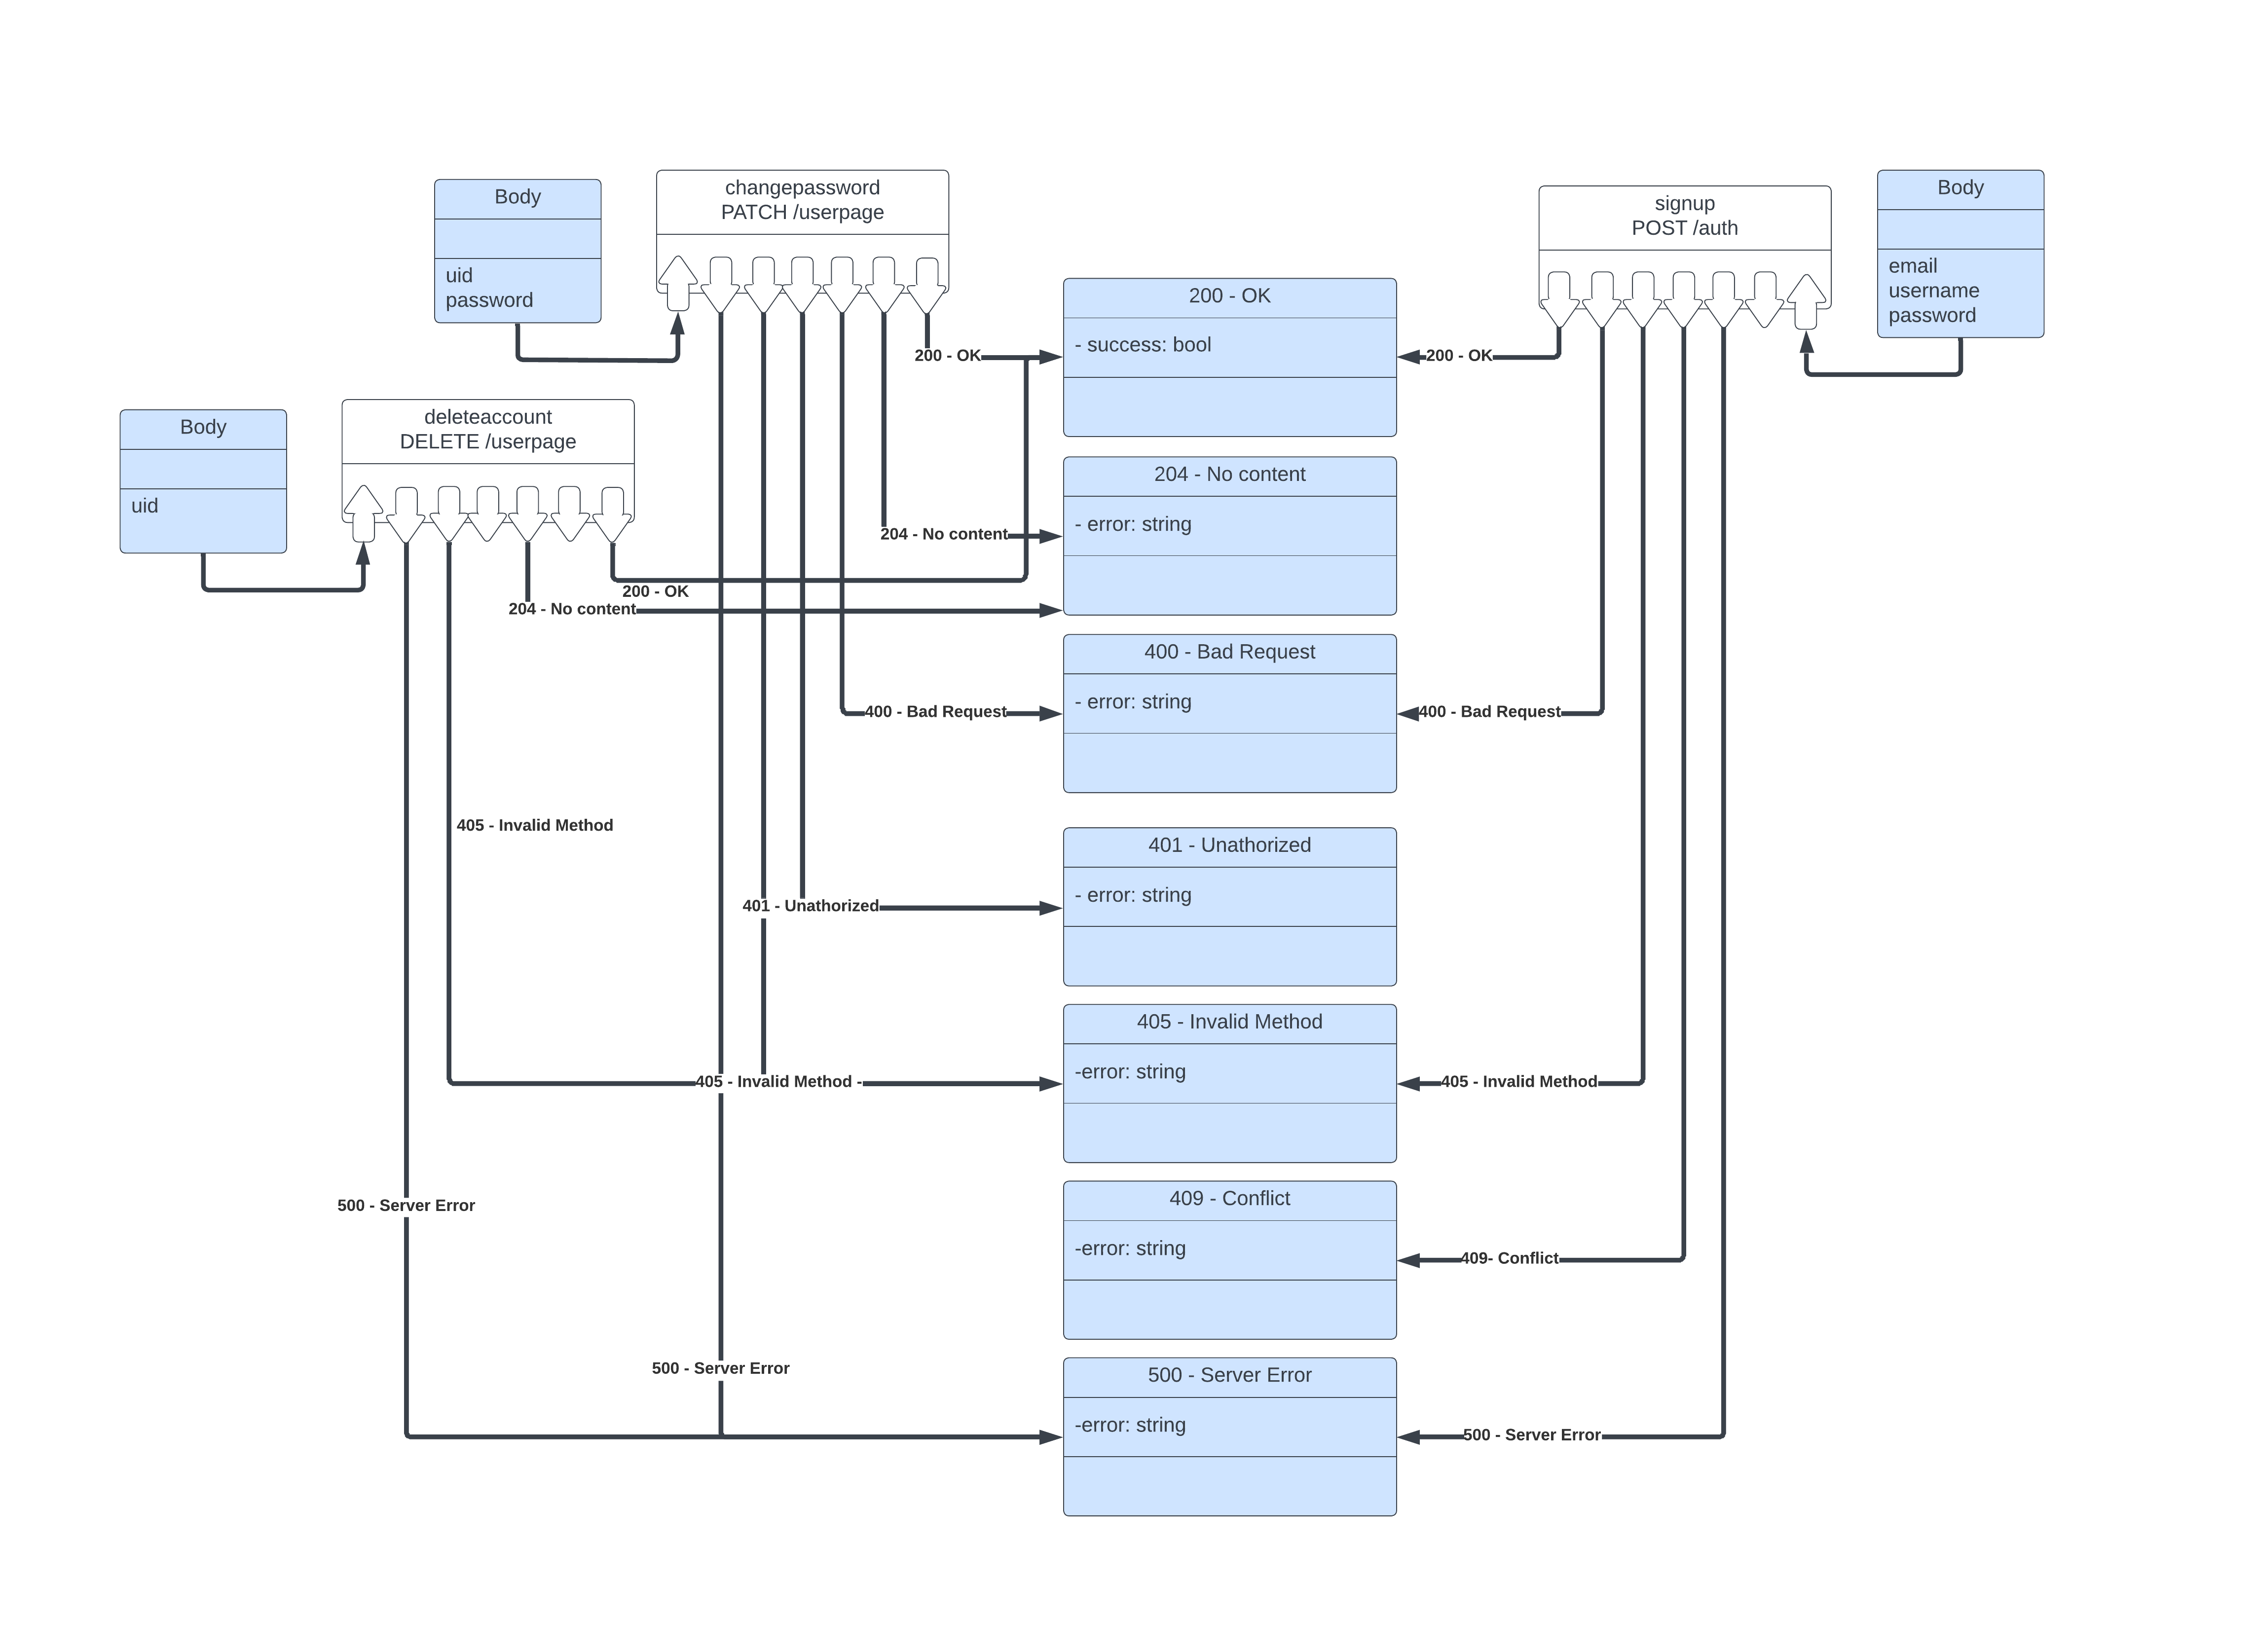
\includegraphics[width=\textwidth]{materiale/Resource Models Users.png}
\newpage
\textbullet \textbf{ Problem API}\\
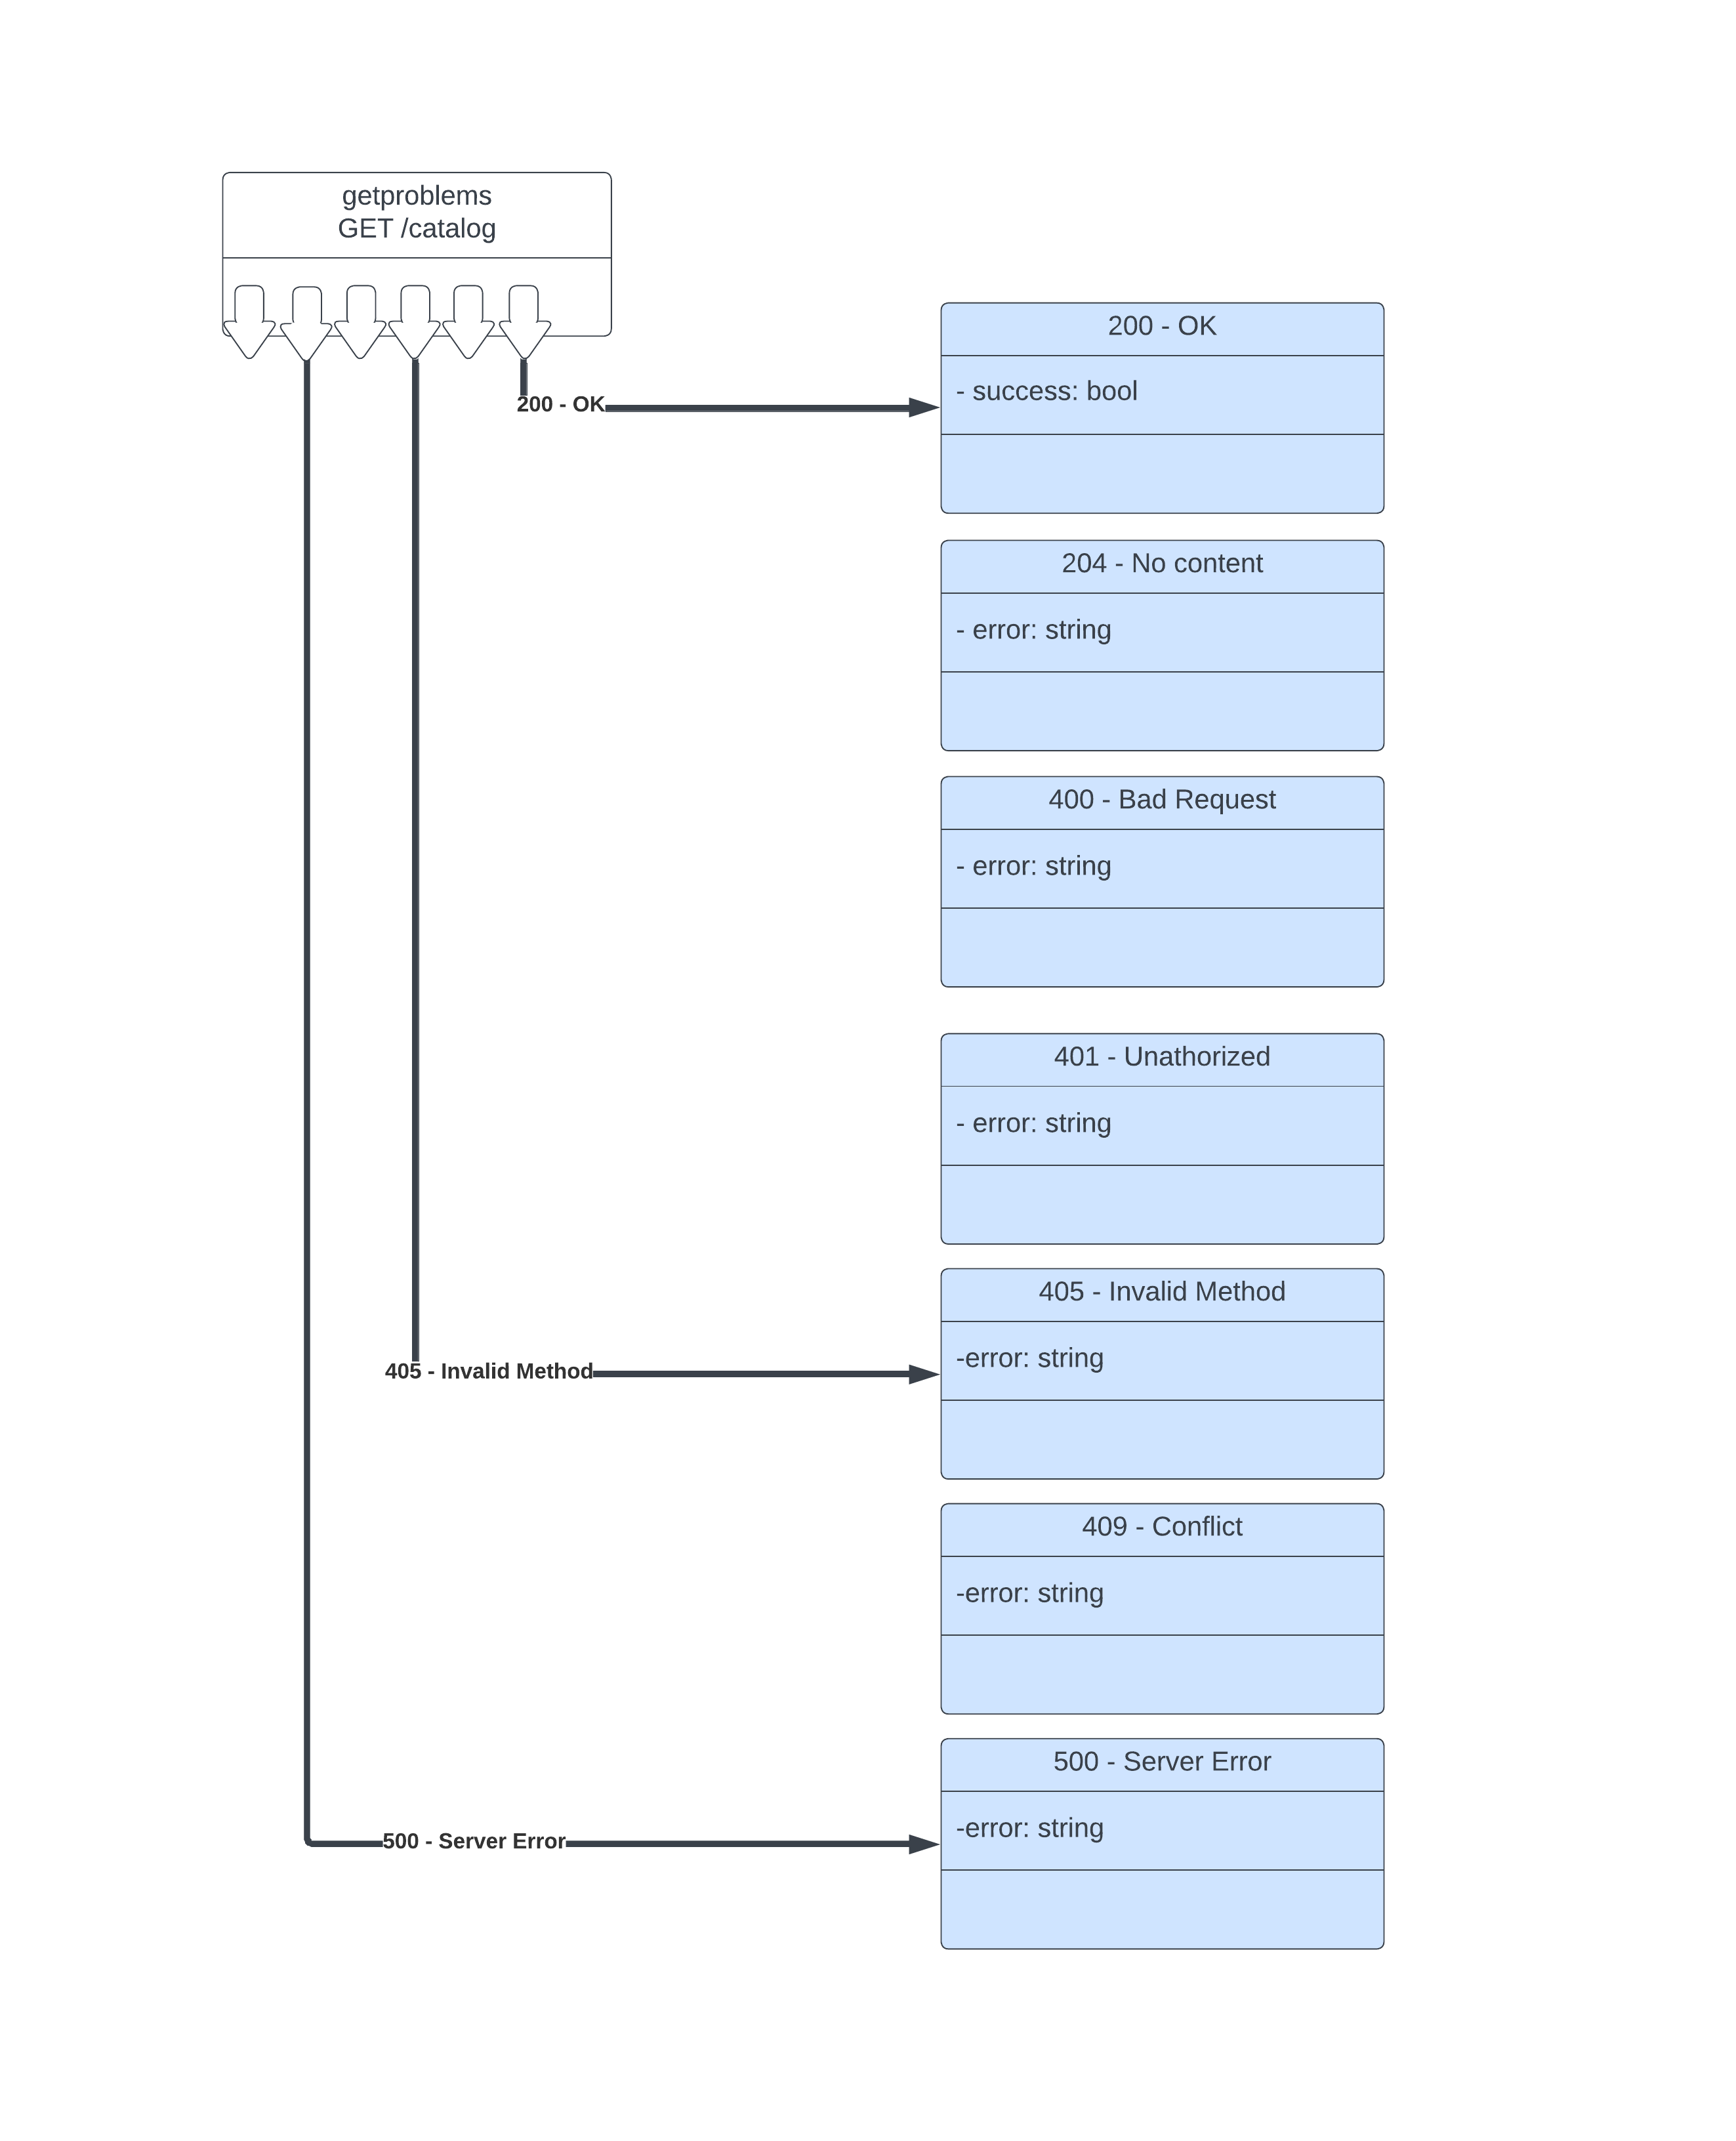
\includegraphics[width=\textwidth]{materiale/Resource Models Problems.png}

\subsection{Sviluppo API}
In questa sezione mostreremo il codice relativo alle API.

\subsubsection{Signup}
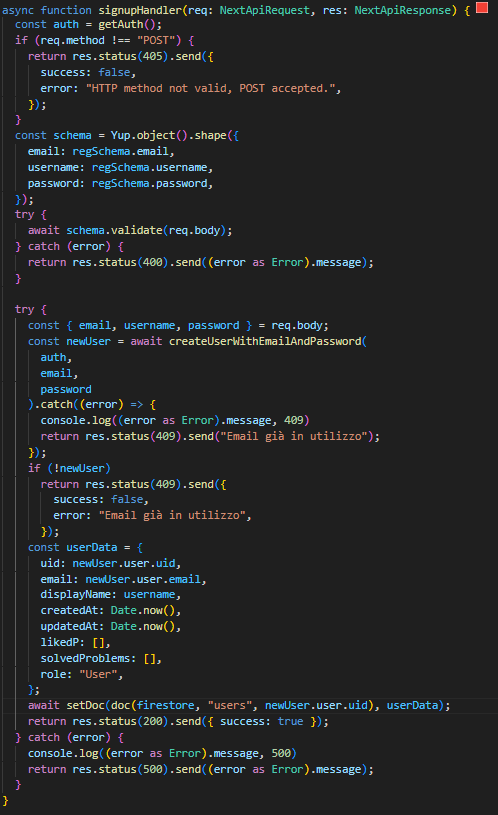
\includegraphics[width=\textwidth,height=19cm]{materiale/API/signup.png}
Questa API permette ad un utente di registrarsi all'interno dell'applicazione, richiede un'email,un username e una password,
attraverso la libreria Yup verificheremo che le informazioni inserite dall'utente siano accettabili, se accettabili, il sistema proverà a registrare l'utente.
In caso abbiamo problemi di conflitto nella creazione dell'utente l'HTTP response avrà come Status Code 409, in caso di una password e/o username malformati avremo uno Status code 400, in caso di un qualsiasi errore non precedentemente previsto
avremo HTTP 500,in caso la richiesta è malformata avremo HTTP 405, e in caso di successo HTTP 200.

\subsubsection{deleteAccount}
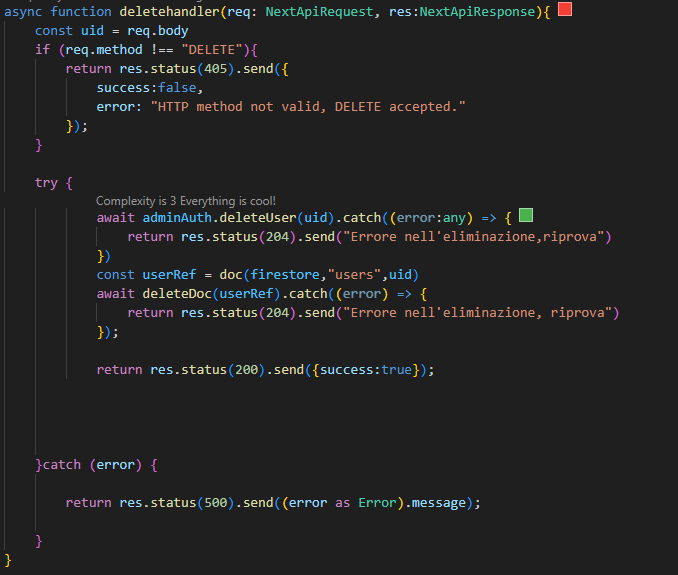
\includegraphics[width=\textwidth]{materiale/API/deleteAccount.png}
\\\\
Questa API permette ad un utente autenticato di eliminare il proprio account e tutti i dati relativi ad esso (ricordiamo che per avere uno storico più accurato i like non verrano rimossi dai problemi),dopo che la richiesta
è stata ricevuta elimineremo prima l'account dell'utente e successivamente tutti i dati contenuti nel database.
In caso la richiesta sia malformata avremo HTTP 405, in caso di problemi (come utente inesistente e/o già eliminato) avremo HTTP 204,in caso di problemi col server avremo HTTP 500, e in caso di successo HTTP 200

\subsubsection{changePassword}
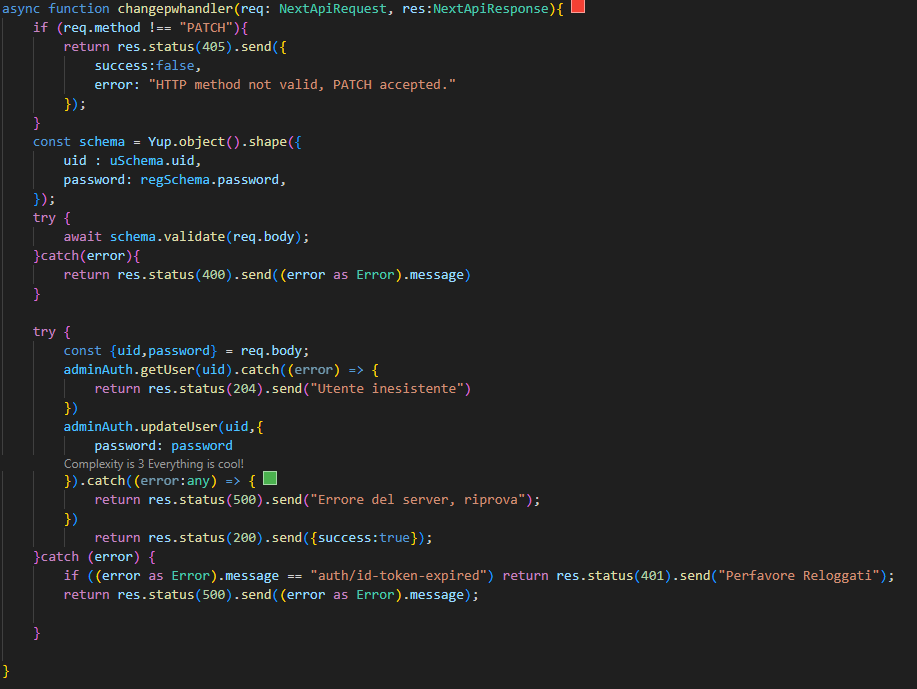
\includegraphics[width=\textwidth]{materiale/API/ChangePassword.png}
\\\\
Questa API permette all'utente di modificare la propria password, sempre che rispetti i requisiti per essere password.
Dopo aver Ricevuto una richiesta, controlleremo se la password rispetta i requisiti per essere tale, dopodichè controlleremo l'esistenza dell'utente e, se esso esiste cambieremo la password con quella fornita.
In caso la richiesta sia malformata avremo HTTP 405,in caso la password fornite sia malformata avremp HTTP 400, in caso di utente inesistente avremo HTTP 204, in caso qualcosa vada storto con l'operazione di modifica
avremo HTTP 500, e in caso di successo HTTP 200.

\subsubsection{getProblems}
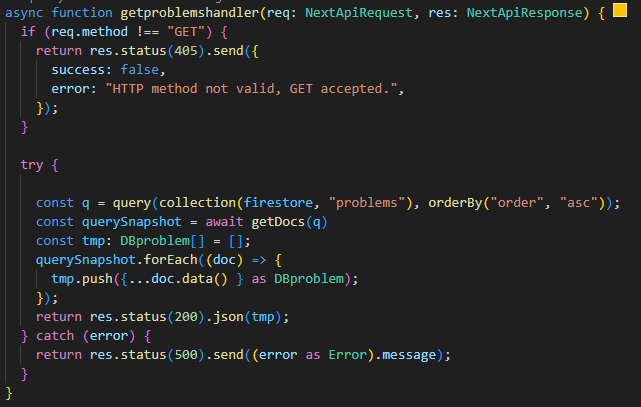
\includegraphics[width=\textwidth]{materiale/API/GetProblems.png}
Questa API resistuisce i problemi disponibili al momento della richiesta e tutti i dati relativi ad essi (ordine,titolo,difficoltà,videoId,categoria ecc).
Dopo aver ricevuto una richiesta manderemo una query al Firestore per ottenere i dati relativi a tutti i problemi presenti nella collection problems.
In caso la richiesta è malformata avremo HTTP 405, in caso la richiesta incontri qualsiasi problema durante la query avremo HTTP 500, in caso di successo HTTP 200.
\newpage
\subsection{Documentazione API}
Le API fornite dall'applicativo che sono state presentate nella sezione precedente sono state documente utilizzando il pacchetto NPM \href{https://www.npmjs.com/package/swagger}{Swagger},
,grazie a questo pacchetto siamo riusciti a generare una pagina web dedicata alla definizione delle specifiche OpenAPI, la quale è disponibile attraverso questo link: \href{https://sleepcode-dev.vercel.app/api-doc}{api-doc}.
In caso la documentazione è disponibile nel codice sorgente.

Durante lo sviluppo delle API abbiamo utilizzato diversi metodi:
\begin{itemize}
  \item GET: utilizzato per ottenere dati da un server, non contiene body.
  \item POST: utilizzato per creare risorse su un server.
  \item PATCH: utilizzato per modificare una risorsa su un server.
  \item DELETE: utilizzato per eliminare risorse da un server.
\end{itemize}

Di seguito riportiamo un'immagine della pagina della documentazione:\\\\
\\\\\
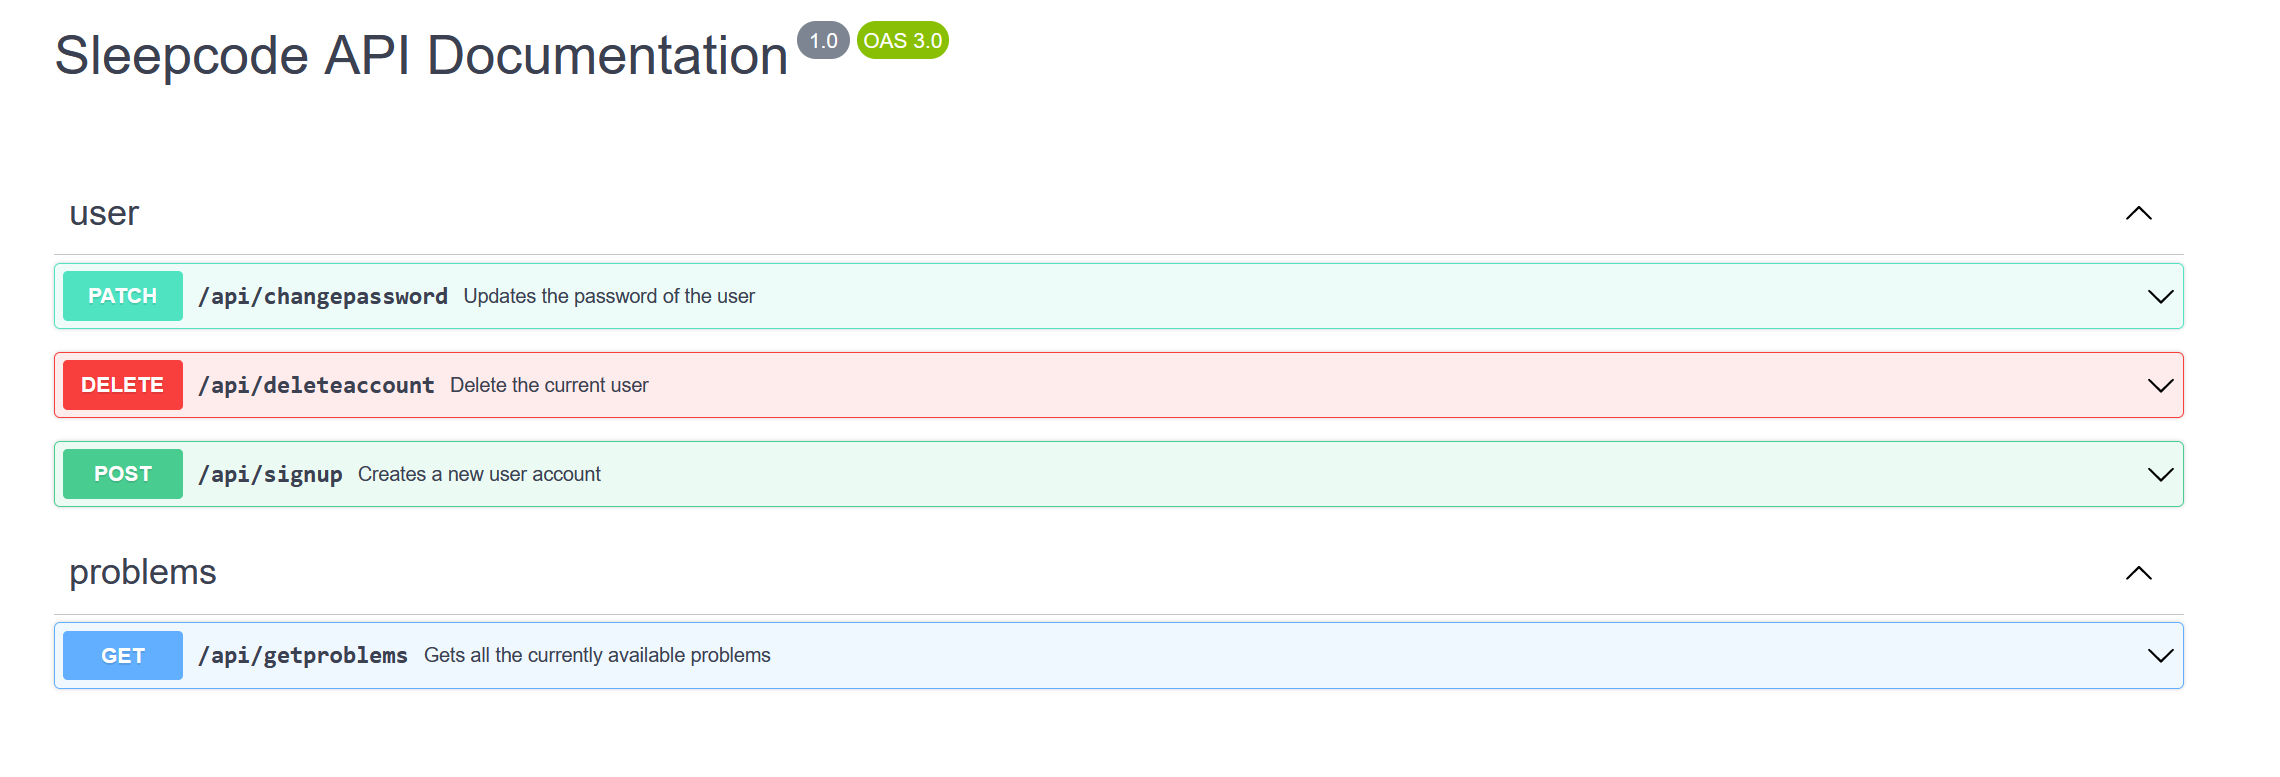
\includegraphics[width=\textwidth]{materiale/API/API-doc.png}

\newpage
\section{Frontend}
In questa sezione del documento mostreremo una parte vitale dell'applicazione, il \textbf{FrontEnd}, ovvero ciò con cui l'utente interagisce con l'applicazione.
Per ogni componente forniremo una breve descrizione delle azioni disponibili all'utente\\\\
\subsection{Home}
La Home è la prima schermata che un utente vede appena si connette al sito dato l'url del sito, essa ha una NavBar (presente in ogni pagina) che contiente diversi bottoni:
\begin{itemize}
  \item Home: Questo bottone, se cliccato riporterà l'utente alla pagina principale.
  \item Catalogo: Questo bottone, se cliccato porterà l'utente alla pagina del catalogo contente tutti i problemi.
  \item Admin Panel: Questo bottone appare solo se nel Database l'utente ha come ruolo "Administrator", ricordiamo che come precedentemente illustrato il ruole di ogni utente è "User" e per promuovere un utente
  si dovrà interagire con la \textbf{CLI} di Firebase per modificare il ruolo del singolo utente, questo può essere fatto solo da persone connesse al progetto sul sito di Firebase.
  \item Pagina Profilo: Questo Bottone appare solo se l'utente è autenticato,se si appoggia il mouse sopra verrà fornite la mail dell'utente attualmente collegato, in caso cliccato si verrà portati alla pagina del profilo utente.
  \item Bottone di Login: Questo bottone compare solo se l'utente non è attualmente autenticato, e se cliccate apre il modello di login.
  \item Bottone di Logout: Questo bottone compare solo se l'utente è autenticato, e se cliccato fa uscire l'utente dall'account.
\end{itemize}
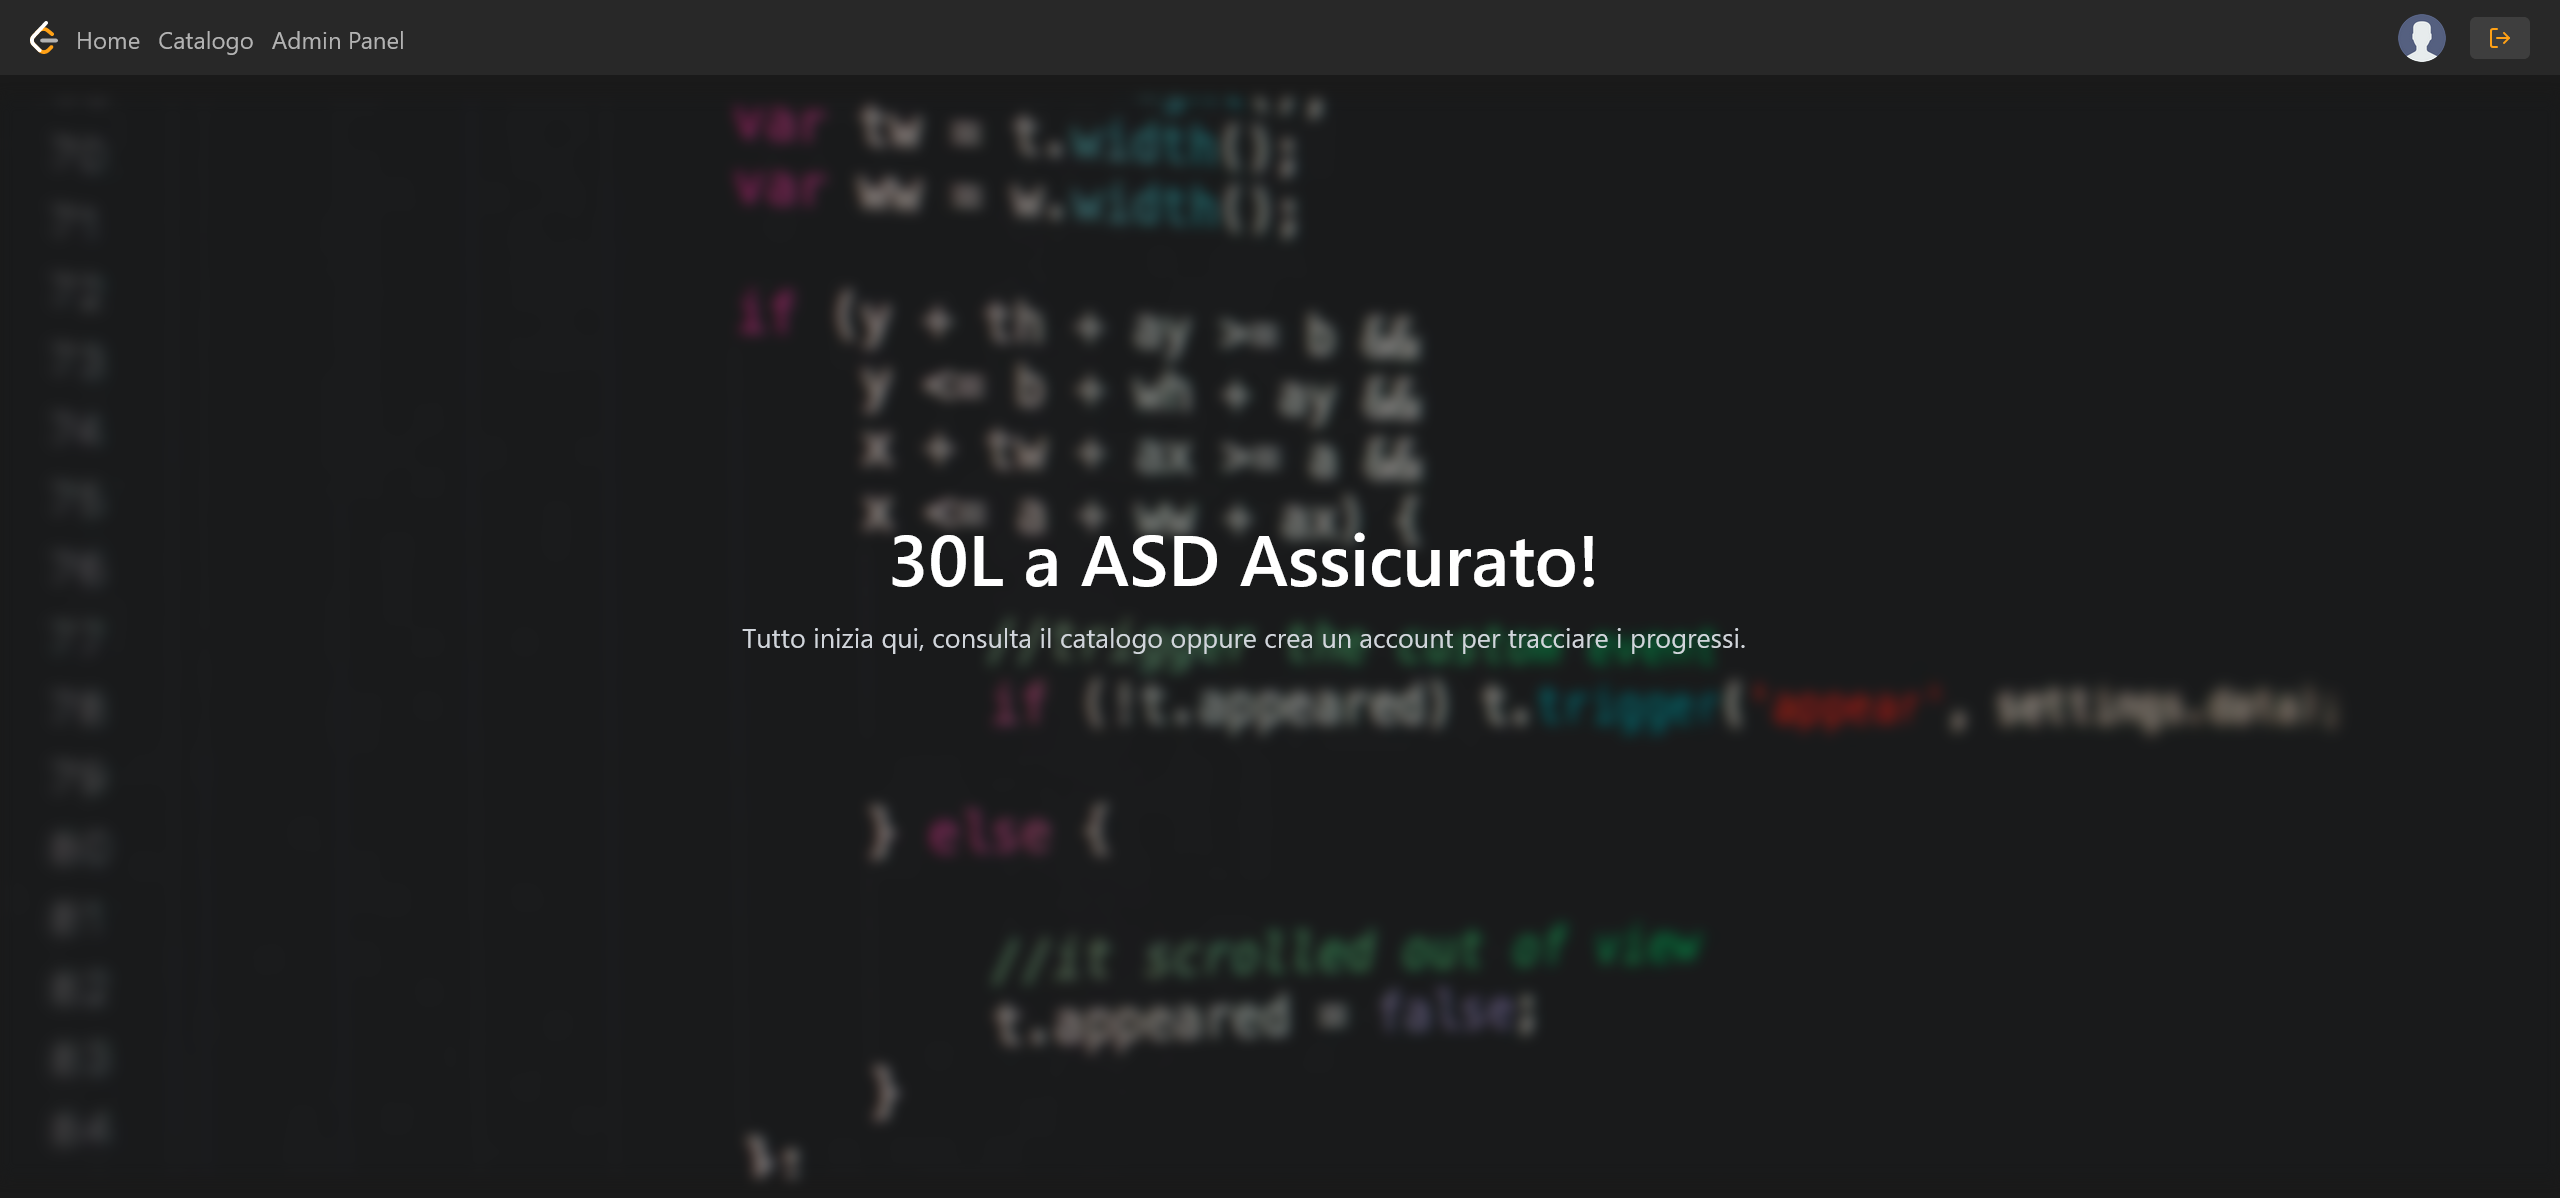
\includegraphics[width=\textwidth]{materiale/sito/Home.png}

\newpage
\subsection{Login}
Questo componente permette ad un utente non ancora autenticato ma registrato di entrare con le proprie credenziali, a causa di regole da firebase non modificabili, la password che viene data non viene controllata se conforme dato che il modello
di recupero password di Firebase non permette l'impostazione di regole per la password strength nel piano gratuito.
Se l'utente ha inserito le proprie credenziali e sono corrette allora verrà autenticato con messaggio di conferma, altrimenti avrà un messaggio di errore.\\\\
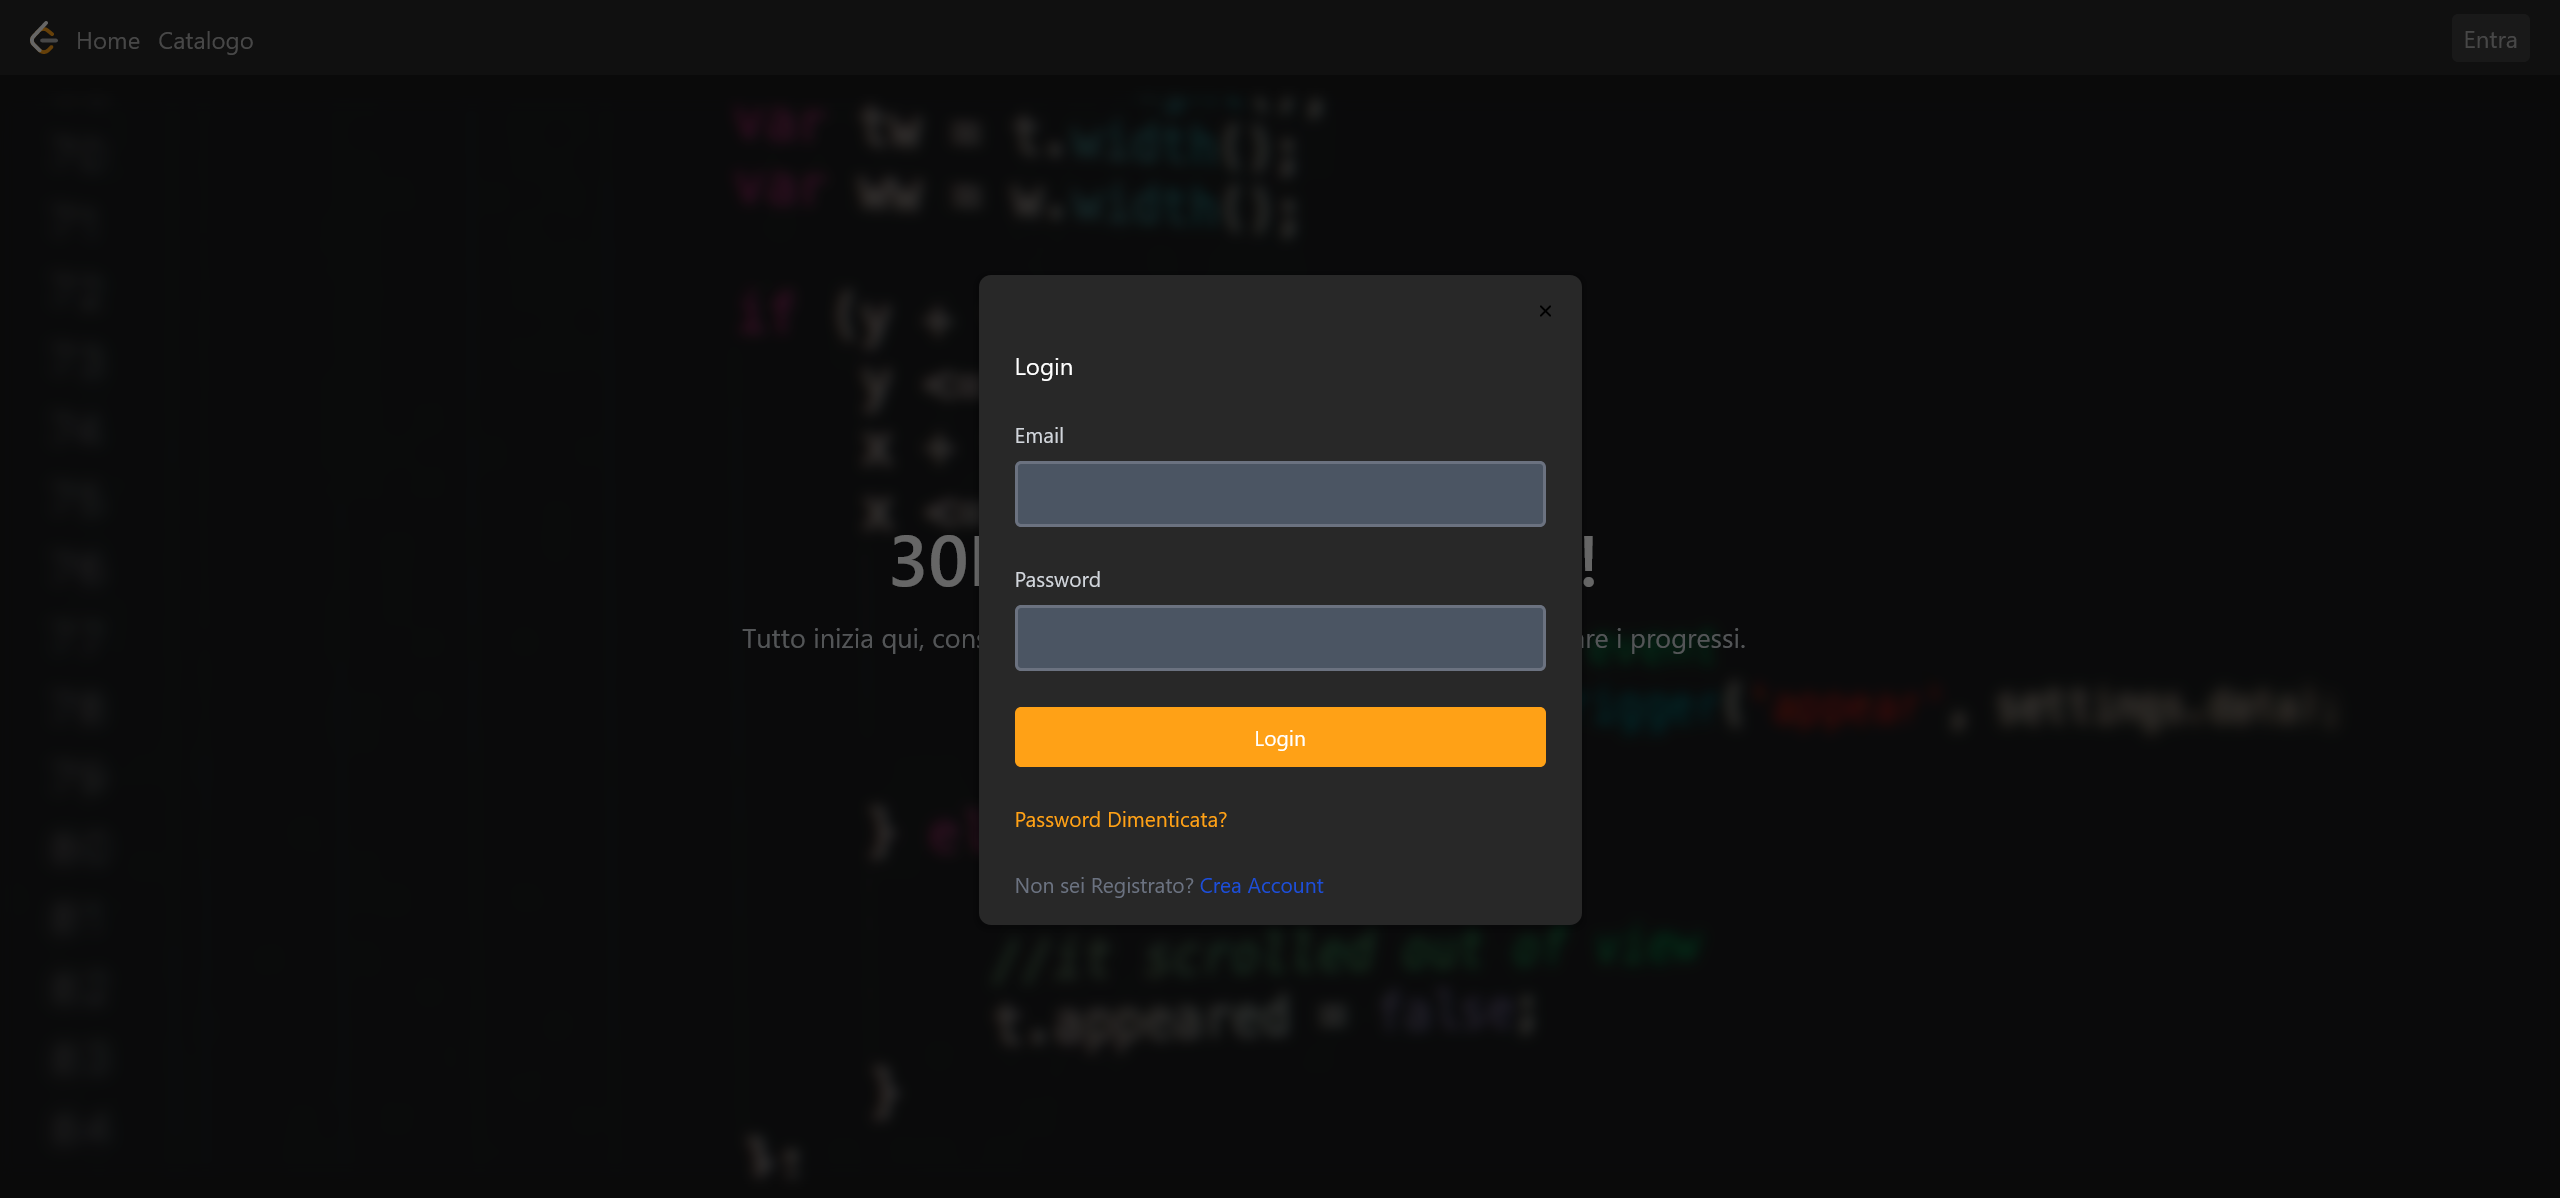
\includegraphics[width=\textwidth]{materiale/sito/Login.png}
\newpage
\subsection{Signup}
Questo componente permette ad un utente non ancora autenticato di registrarsi, l'utente dovrà fornire un'email,username e password, username e password verrano controllati attraverso \textbf{Yup} se rispettano i criteri imposti, in caso contrario l'utente verrà avvertito tramite messagio di errore.
In caso i dati inseriti sono corretti allora l'utente verrà rimandato al componente di Login con messaggio di successo.\\\\
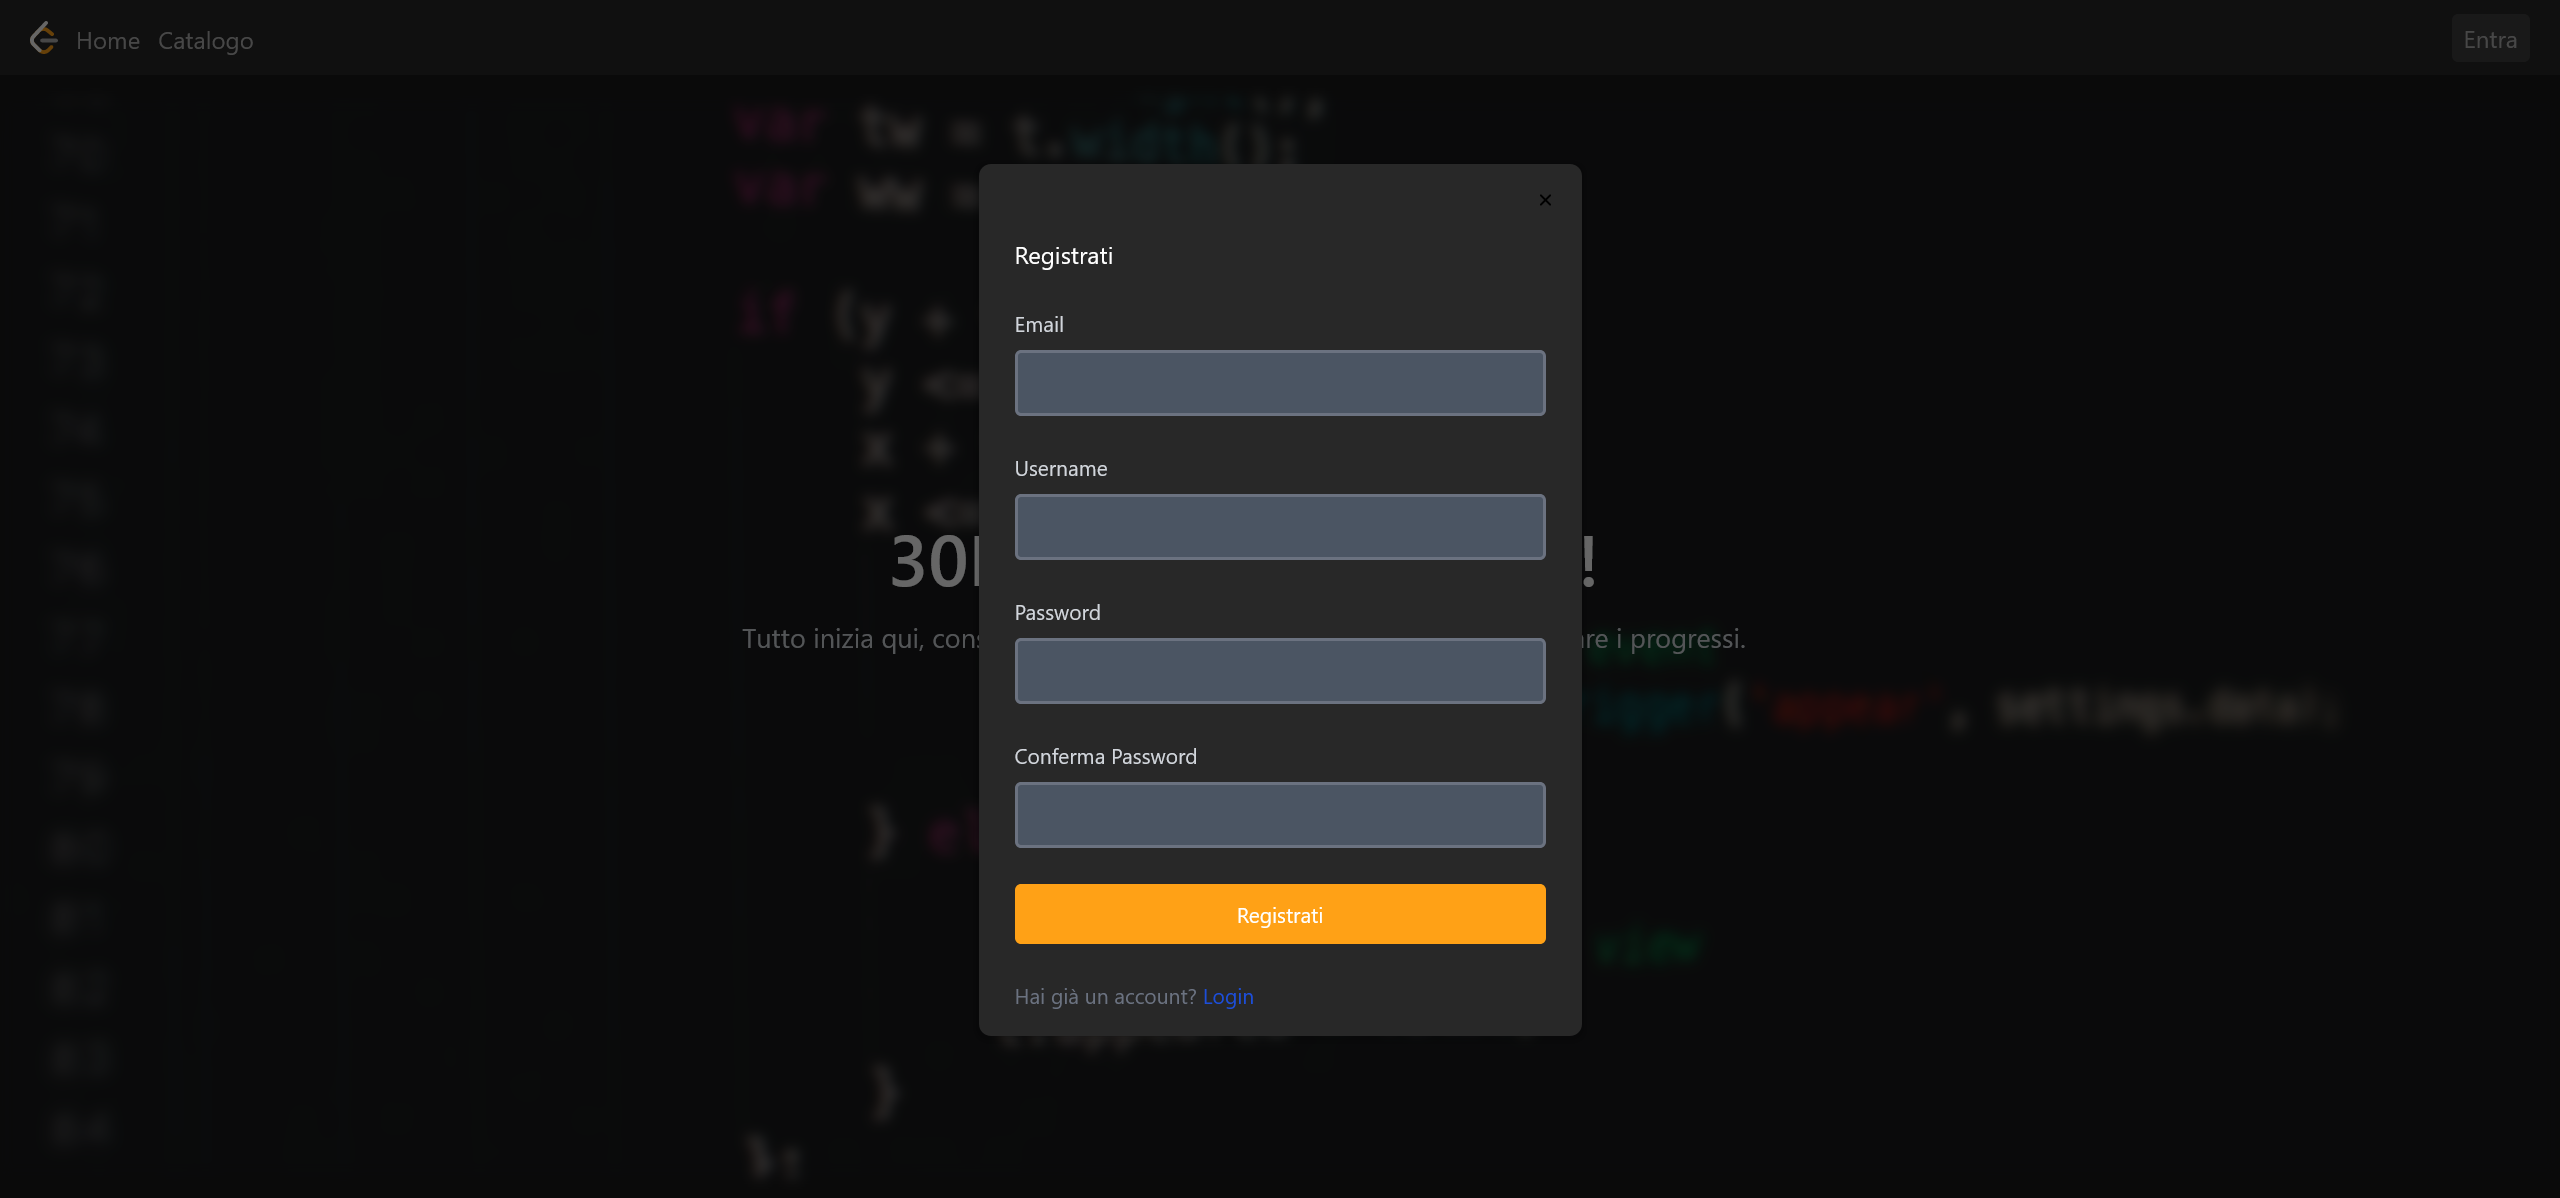
\includegraphics[width=\textwidth]{materiale/sito/Signup.png}
\newpage
\subsection{Recupero Password}
Questo componente permette ad un utente non ancora autenticato di richiedere una mail per recupero password, anche se la mail non è registrata verrà comunque dato un messaggio di conferma di invio, per ragioni di sicurezza. Come già scritto precedentemente
a causa di limitazioni col piano Firebase non possiamo impostare regole per le password "recuperate" in quanto gestite da componenti interni di Firebase non disponibili al nostro piano gratuito.\\\\
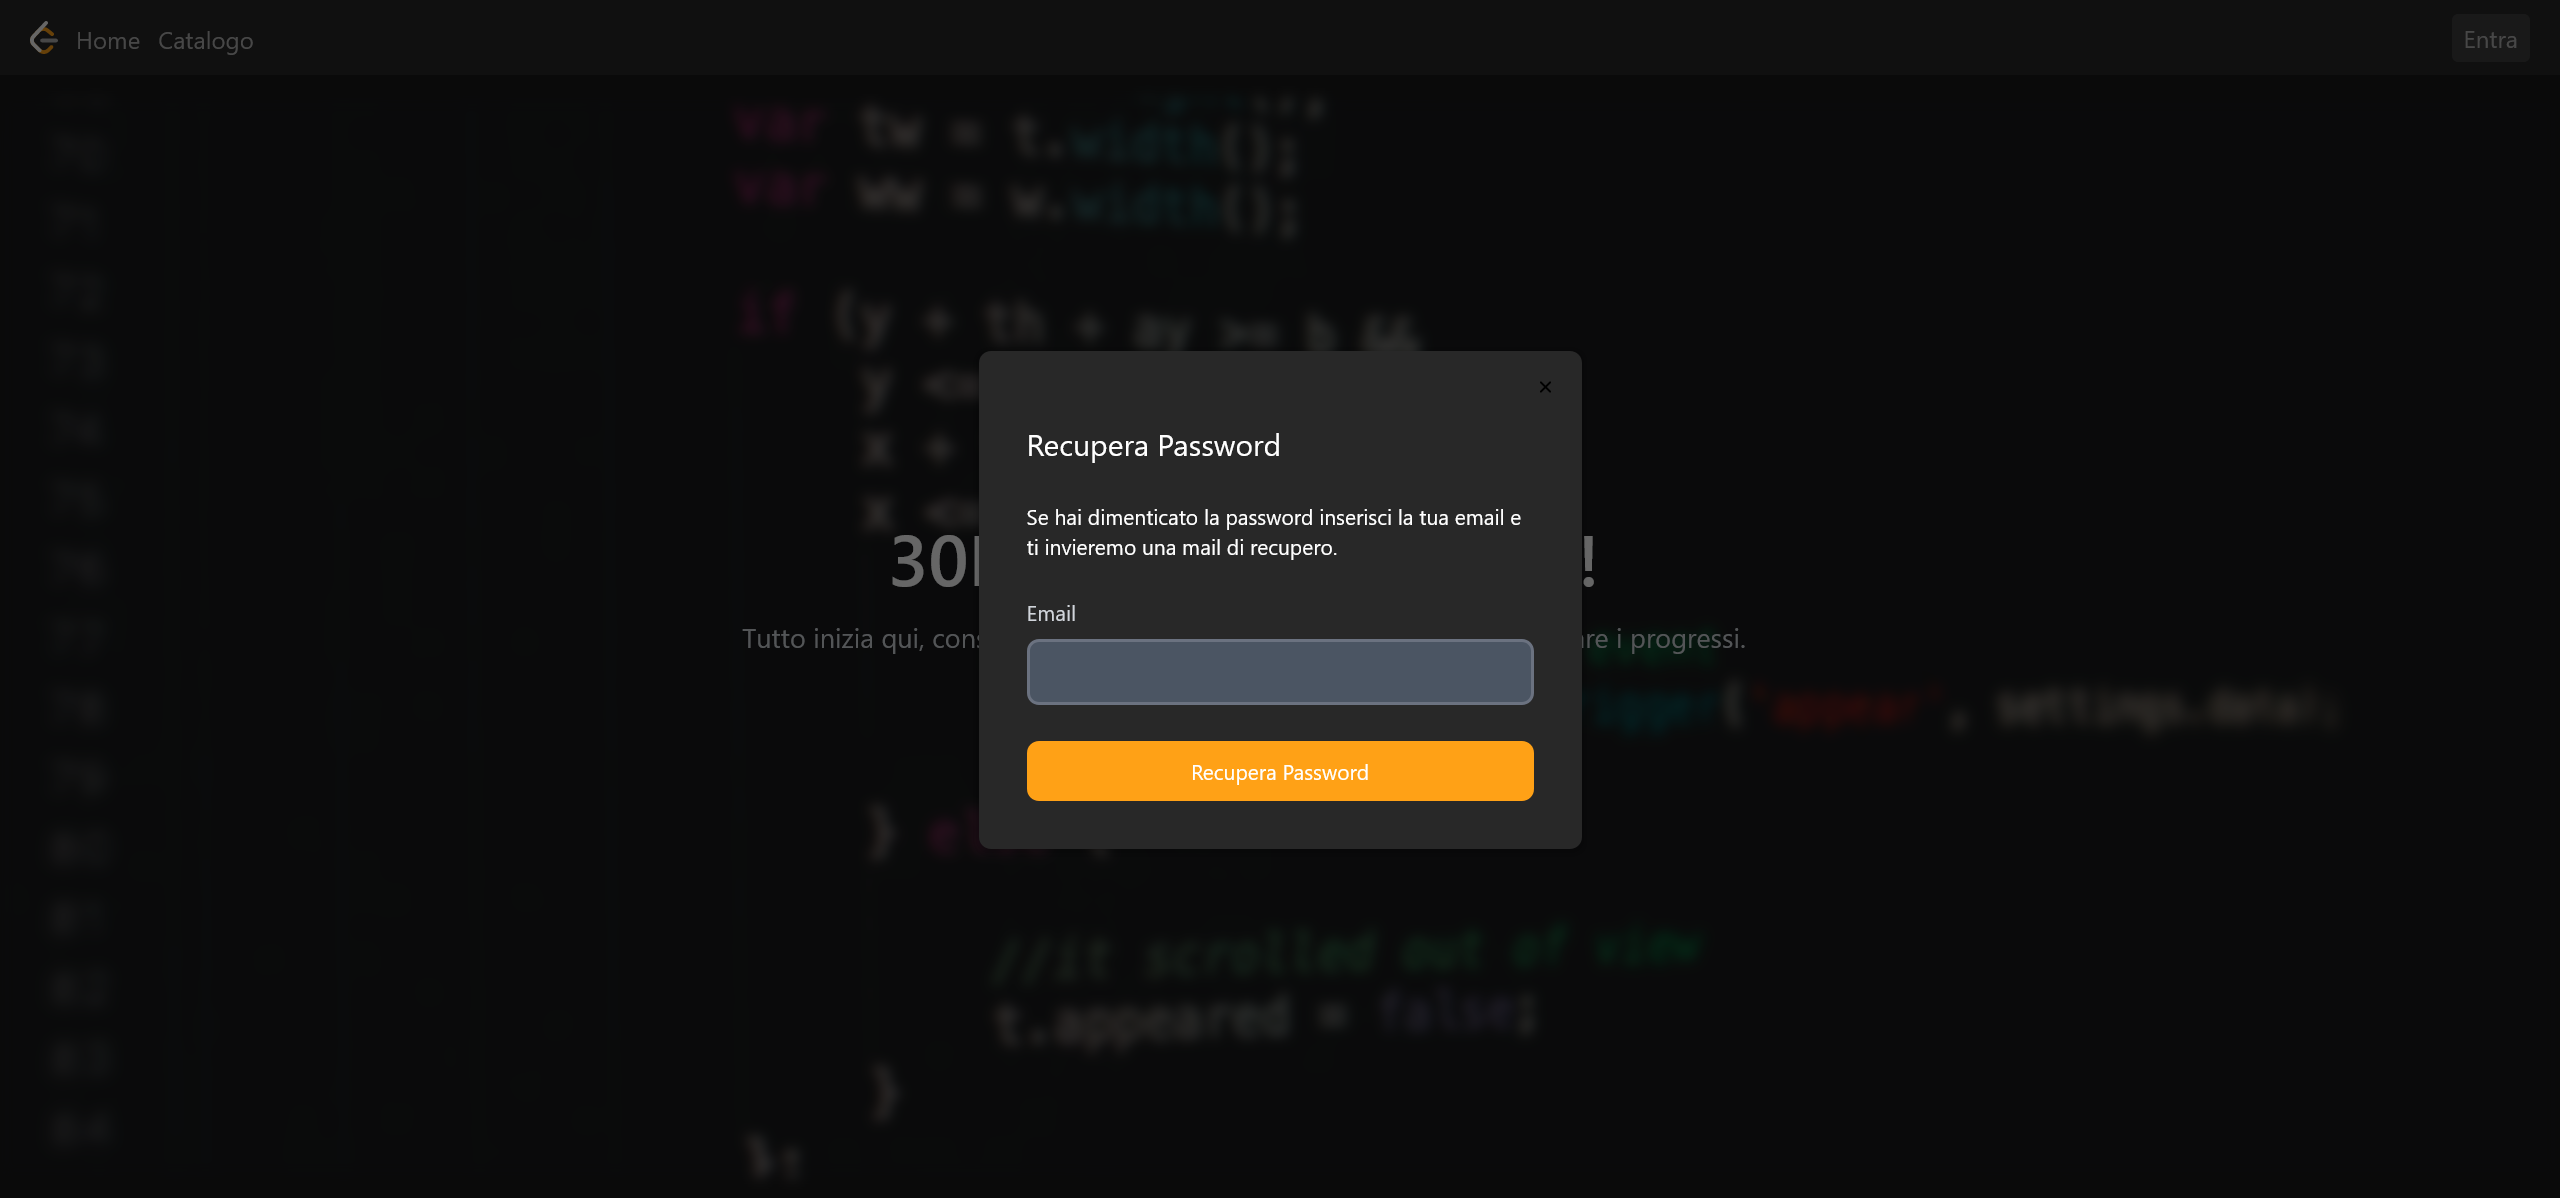
\includegraphics[width=\textwidth]{materiale/sito/Recupero Pw.png}
\newpage
\subsection{Pannelo Admin}
Questo componente (non completamente sviluppata) permette ad un utente amministratore di aggiungere problemi al database, pultroppo per mancanza di tempo non siamo riusciti a sviluppare la funzione in tempo, ci scusiamo per l'incovenienza.\\\\
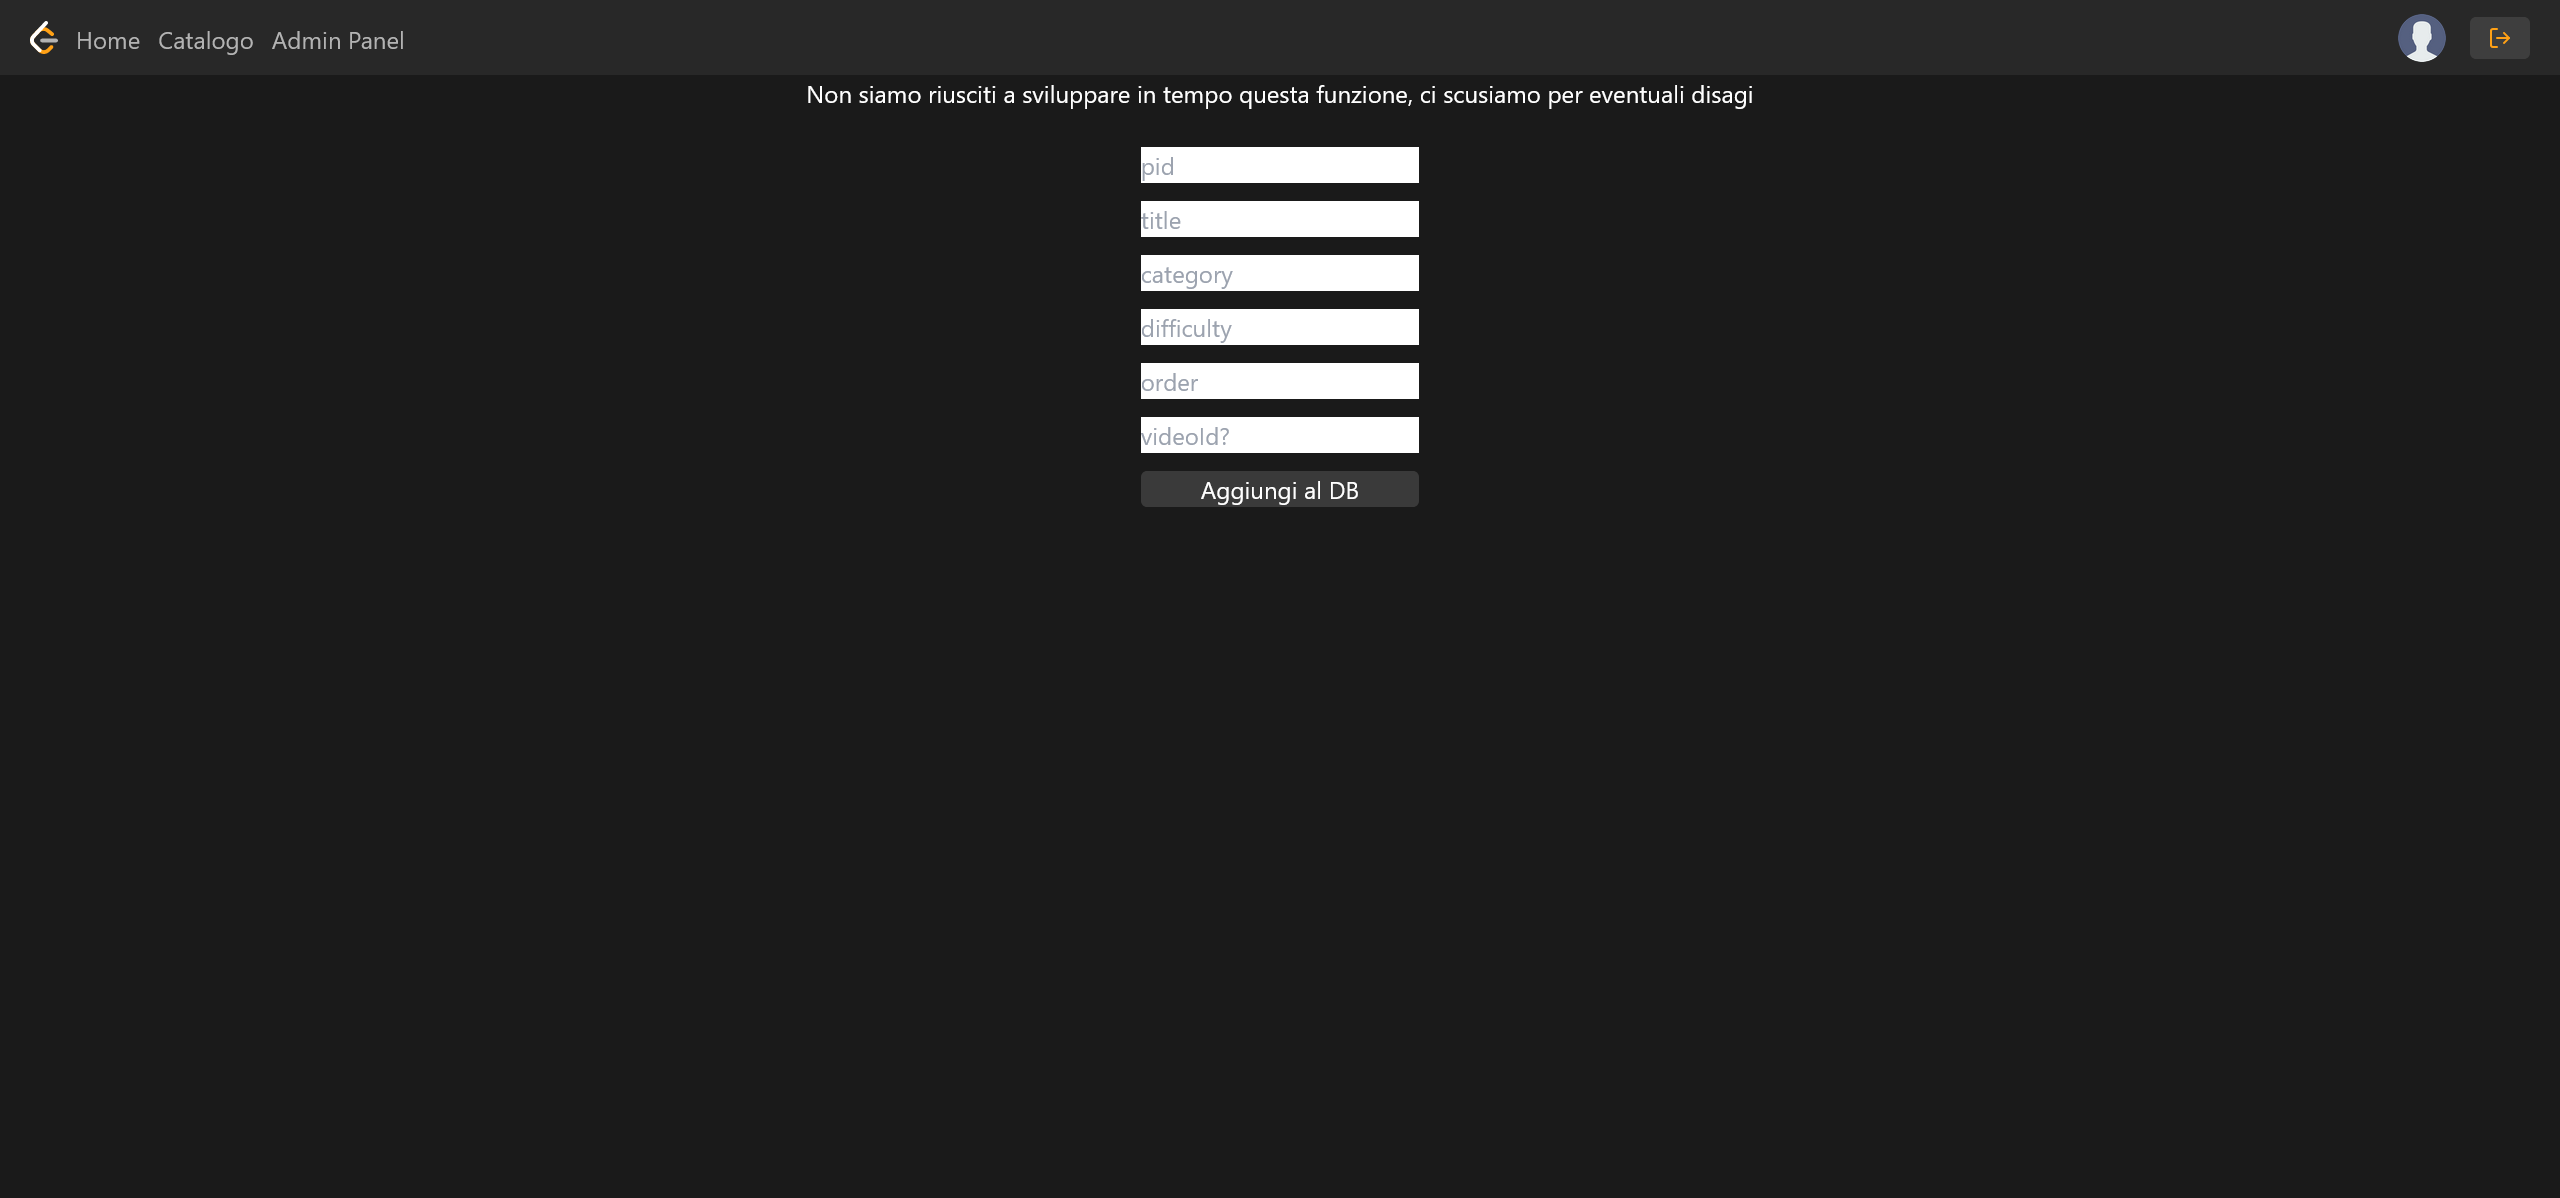
\includegraphics[width=\textwidth]{materiale/sito/Pannello Admin.png}
\newpage
\subsection{Pagina Profilo}
Questa pagina permette ad un utente autenticato di accedere alle funzioni di modifica password e di eliminazione account attraverso appositi form, in caso un utente cerca di accedersi senza essere autenticato verrà riportato alla home.\\\\
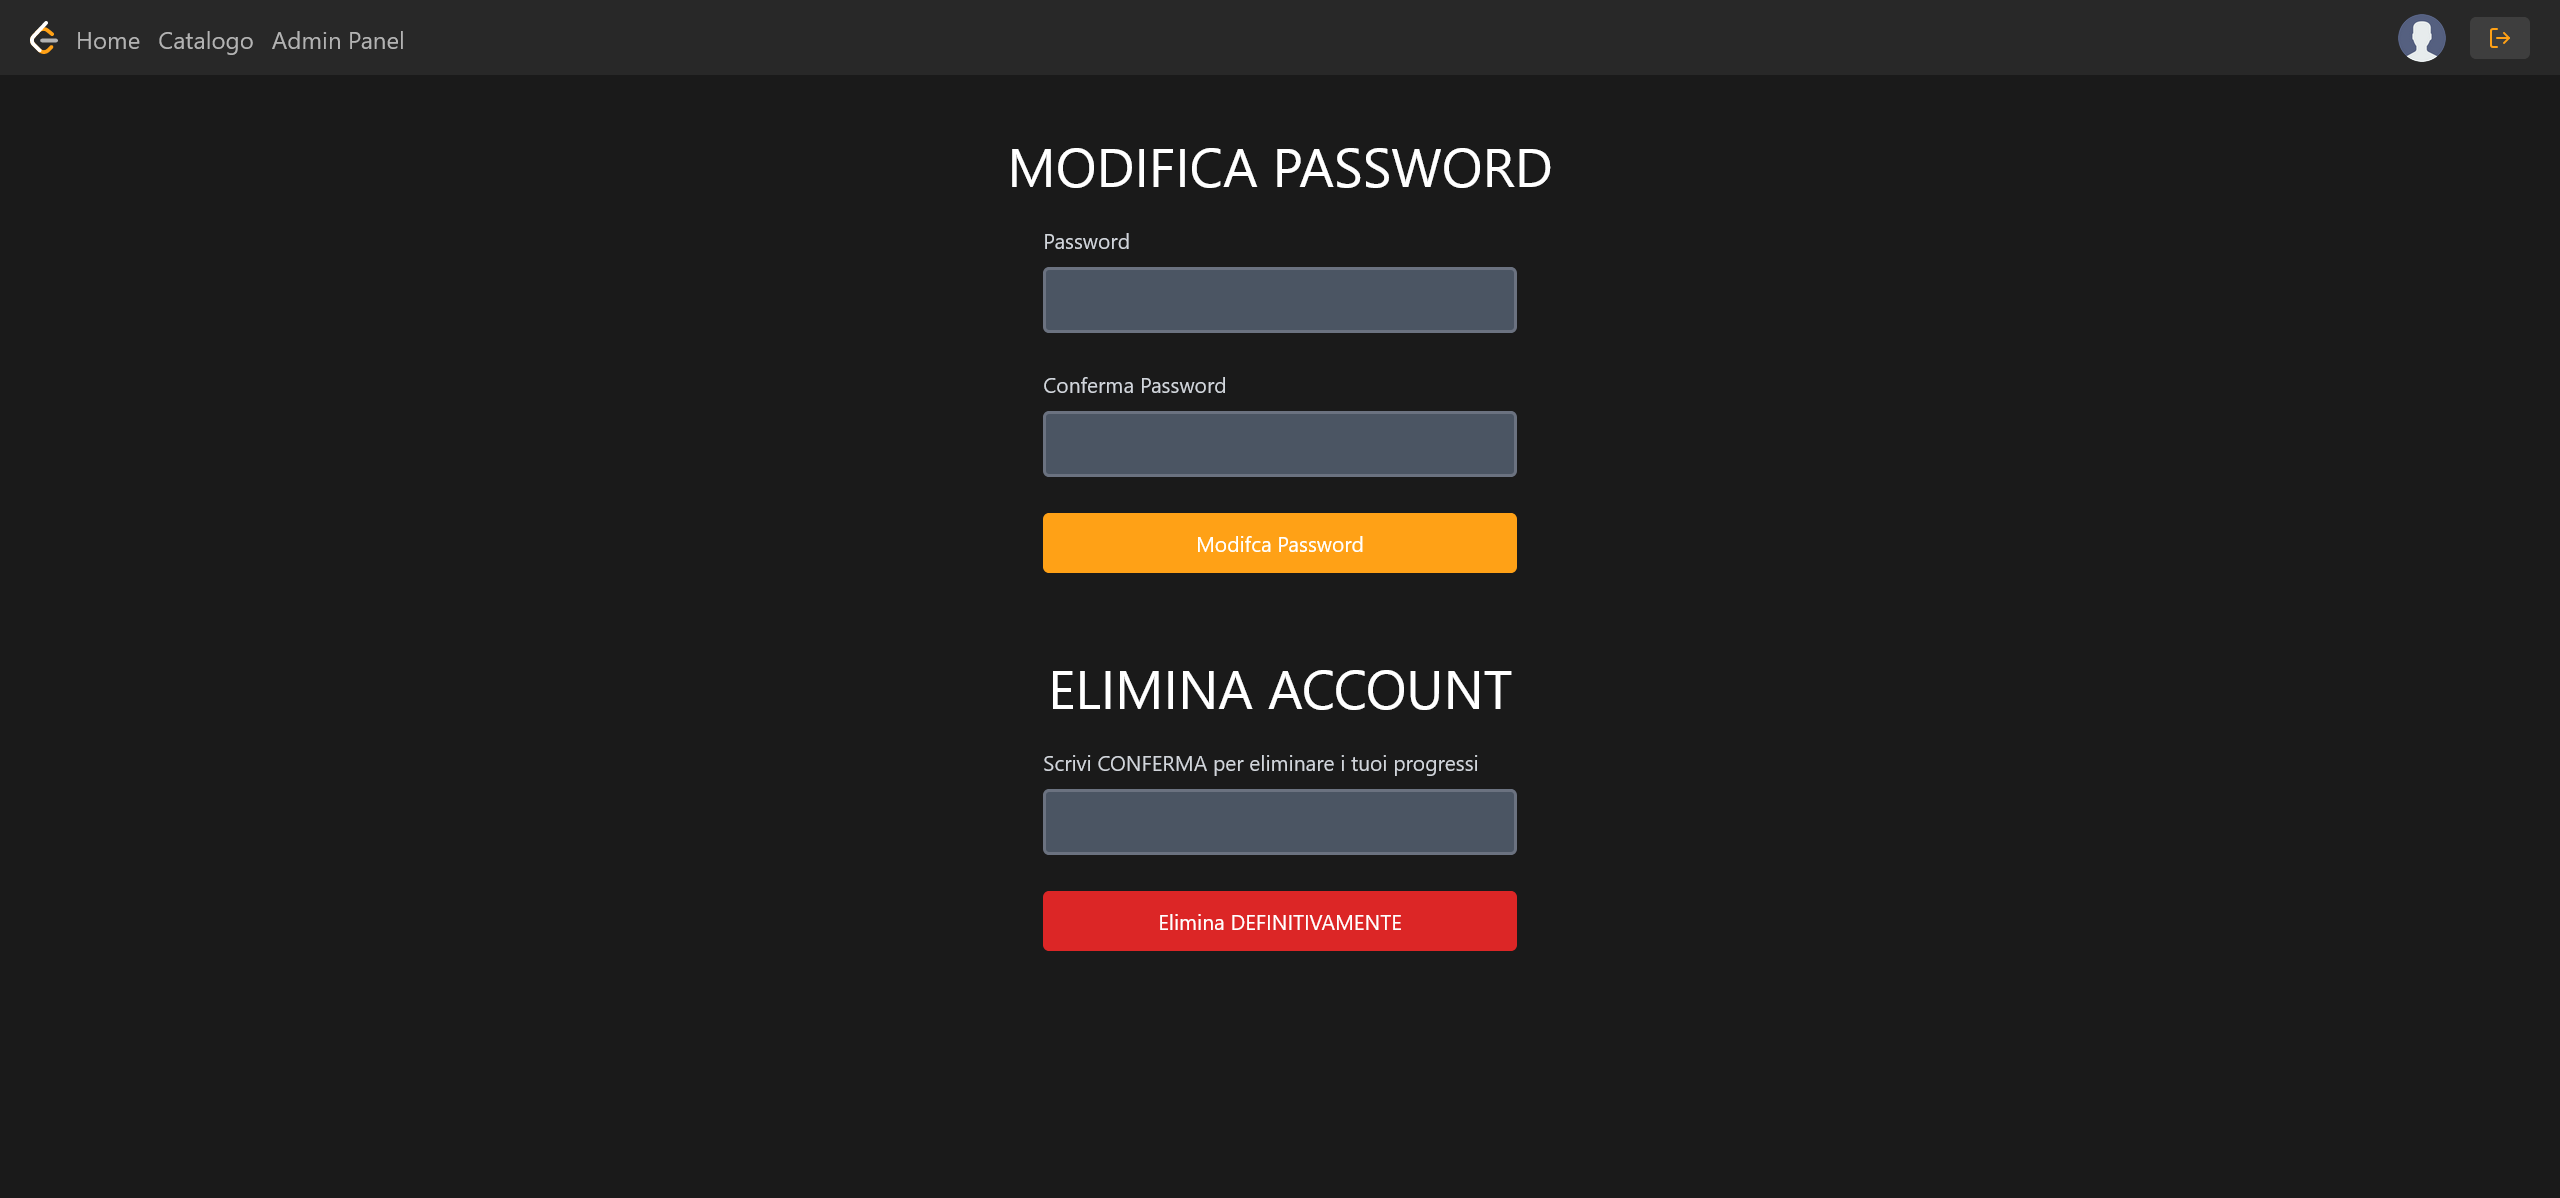
\includegraphics[width=\textwidth]{materiale/sito/Pagina Profilo.png}
\newpage
\subsection{Catalogo}
Questa pagina raccoglie tutti i problemi disponibili, la loro difficoltà,categoria,ordine,titolo,e videoId, e gli offre a tutti gli utenti, in caso l'utente sia autenticato, verrà mostrato un componente che traccia i progressi del singolo utente, e i problemi risolto e/o aggiunti ai preferiti. Oltre a questo un qualsiasi
utente cliccando sull'icona nella colonna "\textbf{Soluzione}" verrà aperta una overlay per visualizzare un video che offre suggerimenti su come risolvere il problema e la soluzione in linguaggio Javascript.
Quando un qualsiasi utente si connette verrano mostrati degli "Scheletri" per mostrare all'utente che la pagina sta aspettando informazioni dal server, e che di conseguenza dovrà aspettare.\\\\
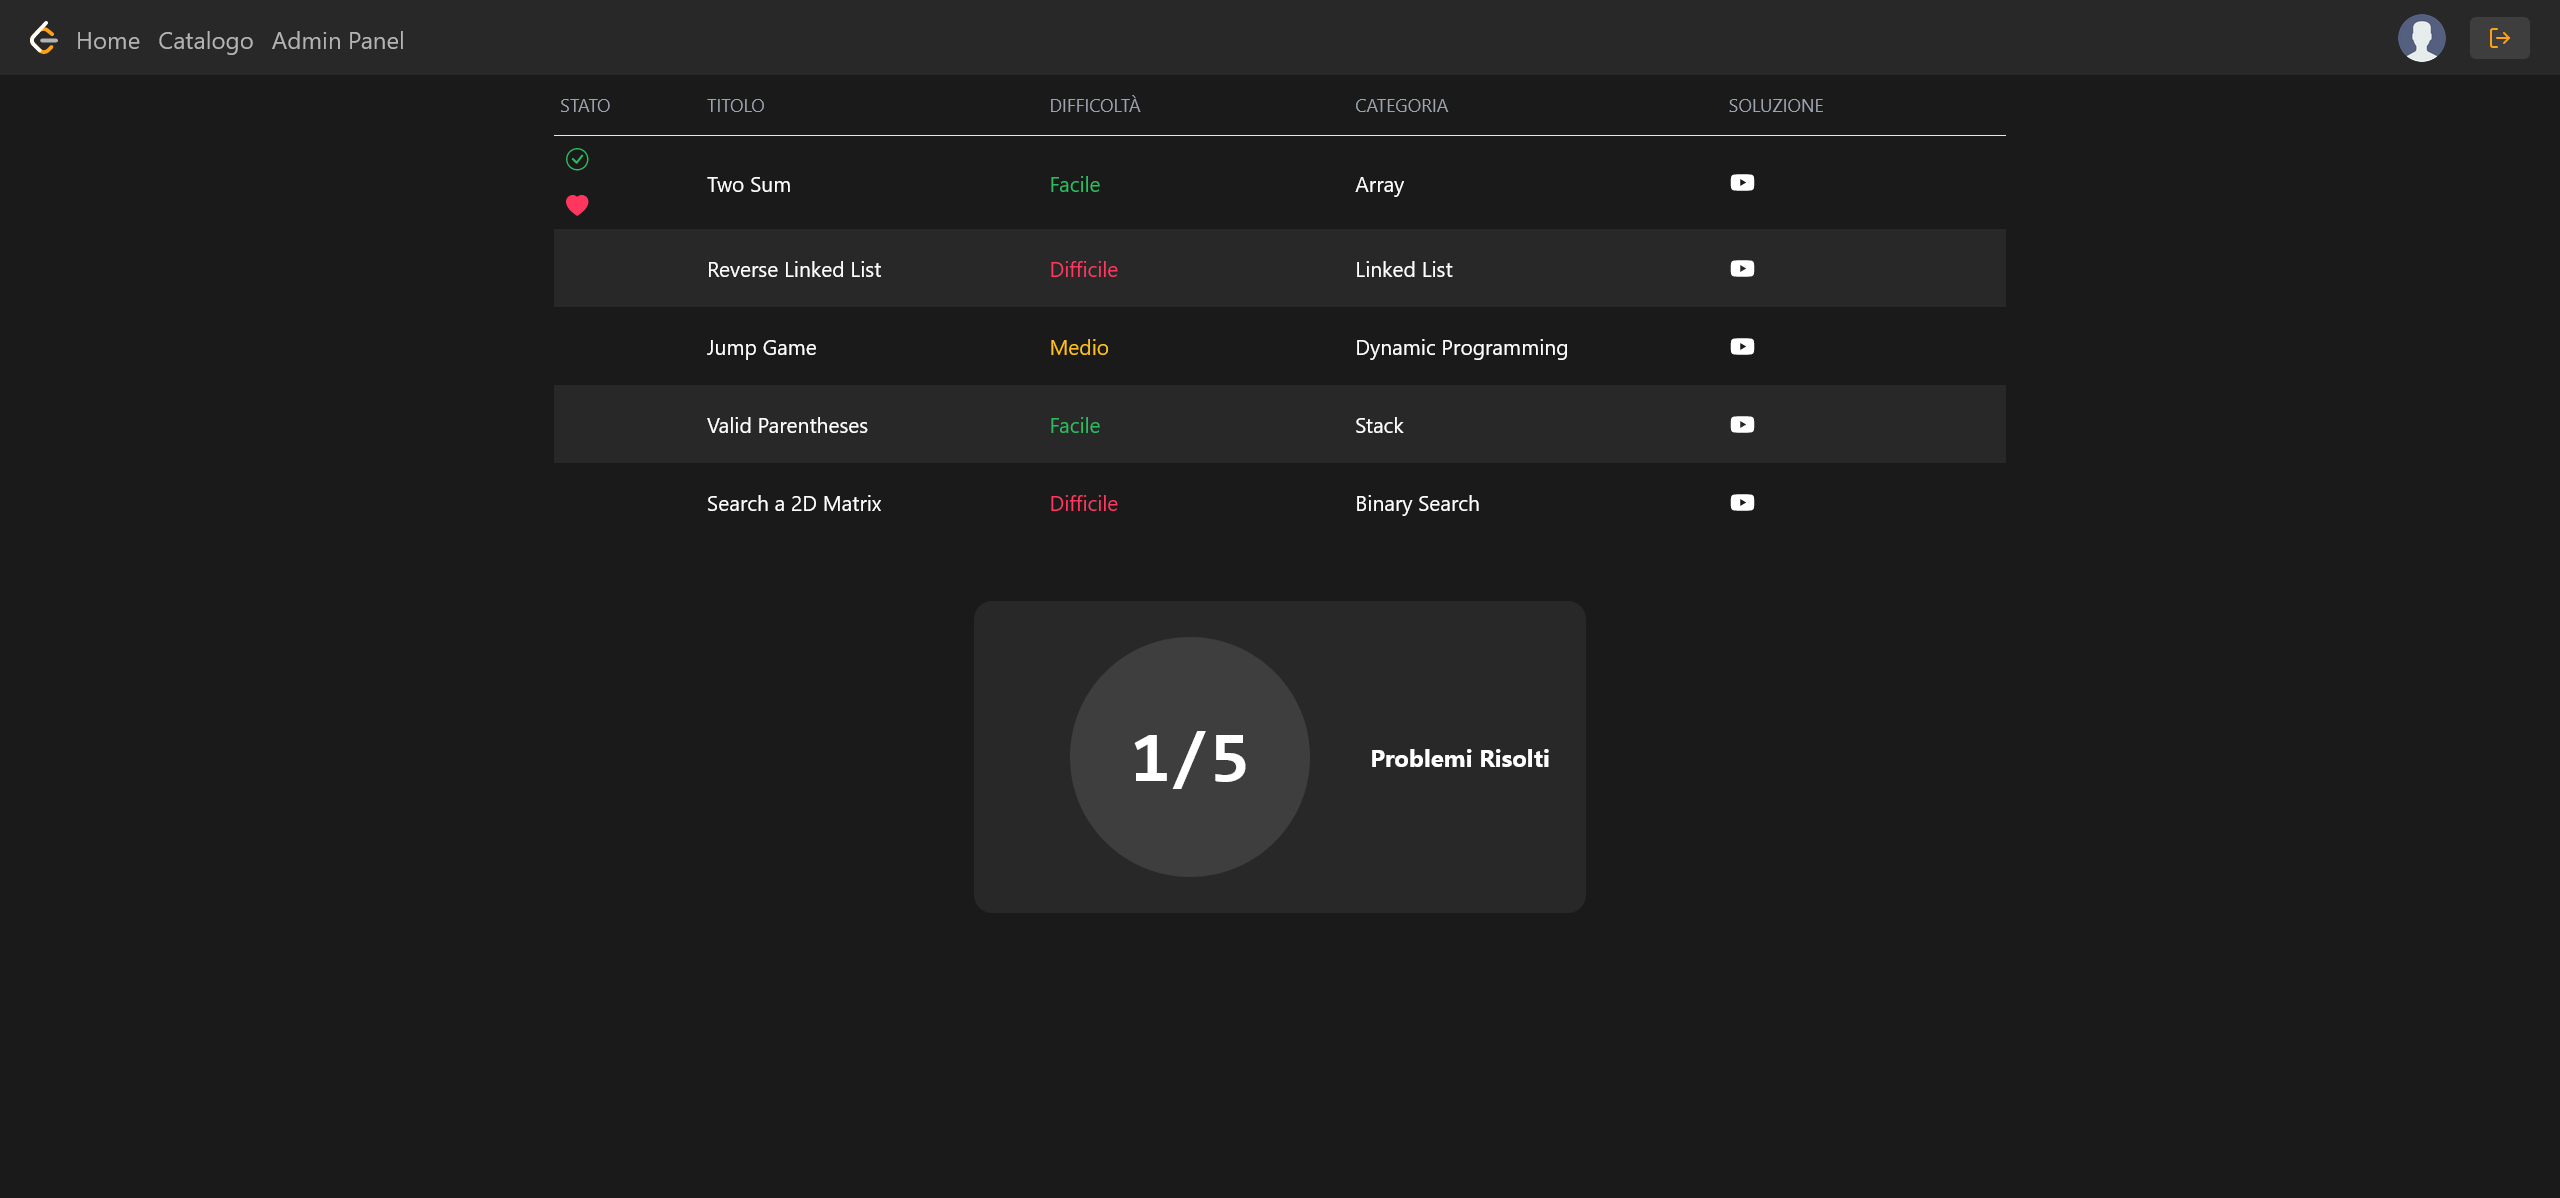
\includegraphics[width=\textwidth]{materiale/sito/Catalogo.png}
\newpage
\subsection{Problema}
Questa pagina esiste per ogni problema al momento disponibile ed è suddivisa in 3 parti:
\begin{itemize}
  \item Descrizione: Contiene tutte le informazioni e/o immagini relative al problema, oltre ad indicaticare e permettere di aggiungere un problema ai preferiti e visualizzare il numero di "like" e capire se il problema è gia stato risolto. Oltre a questo abbiamo un numero variabile di esempi per aiutare l'utente nella risoluzione del problema.
  \item Console: Dove l'utente può scrivere codice e selezionare il linguaggio con cui risolvere il problema, al momento l'unico linguaggio disponibile è Javascript, siccome altri linguaggi richiederebbero server dedicati per la compilazione del file. Ricordiamo di non modificare la firma della funziona.
  \item Testcase: Dove l'utente è in grado di selezione quale test case vedere e sottomettere o provare a risolvere il problema attraverso appositi bottoni. (\textbf{Sottometti o Runna})
\end{itemize}
Oltre a questo ogni utente (anche non autenticato) è in grado di cliccare sull'icona a forma di orologio e cronometrare il proprio tempo di risoluzione del problema, il fermare o resettare il cronometro è compito dell'utente.\\\\
In caso l'utente connesso alla pagina non è autenticato esso non potrà tracciare i propri progressi nè aggiungere problemi ai preferiti, in caso si prova a eseguire quest'ultima azione verrà riportato un messaggio di errore.\\\\
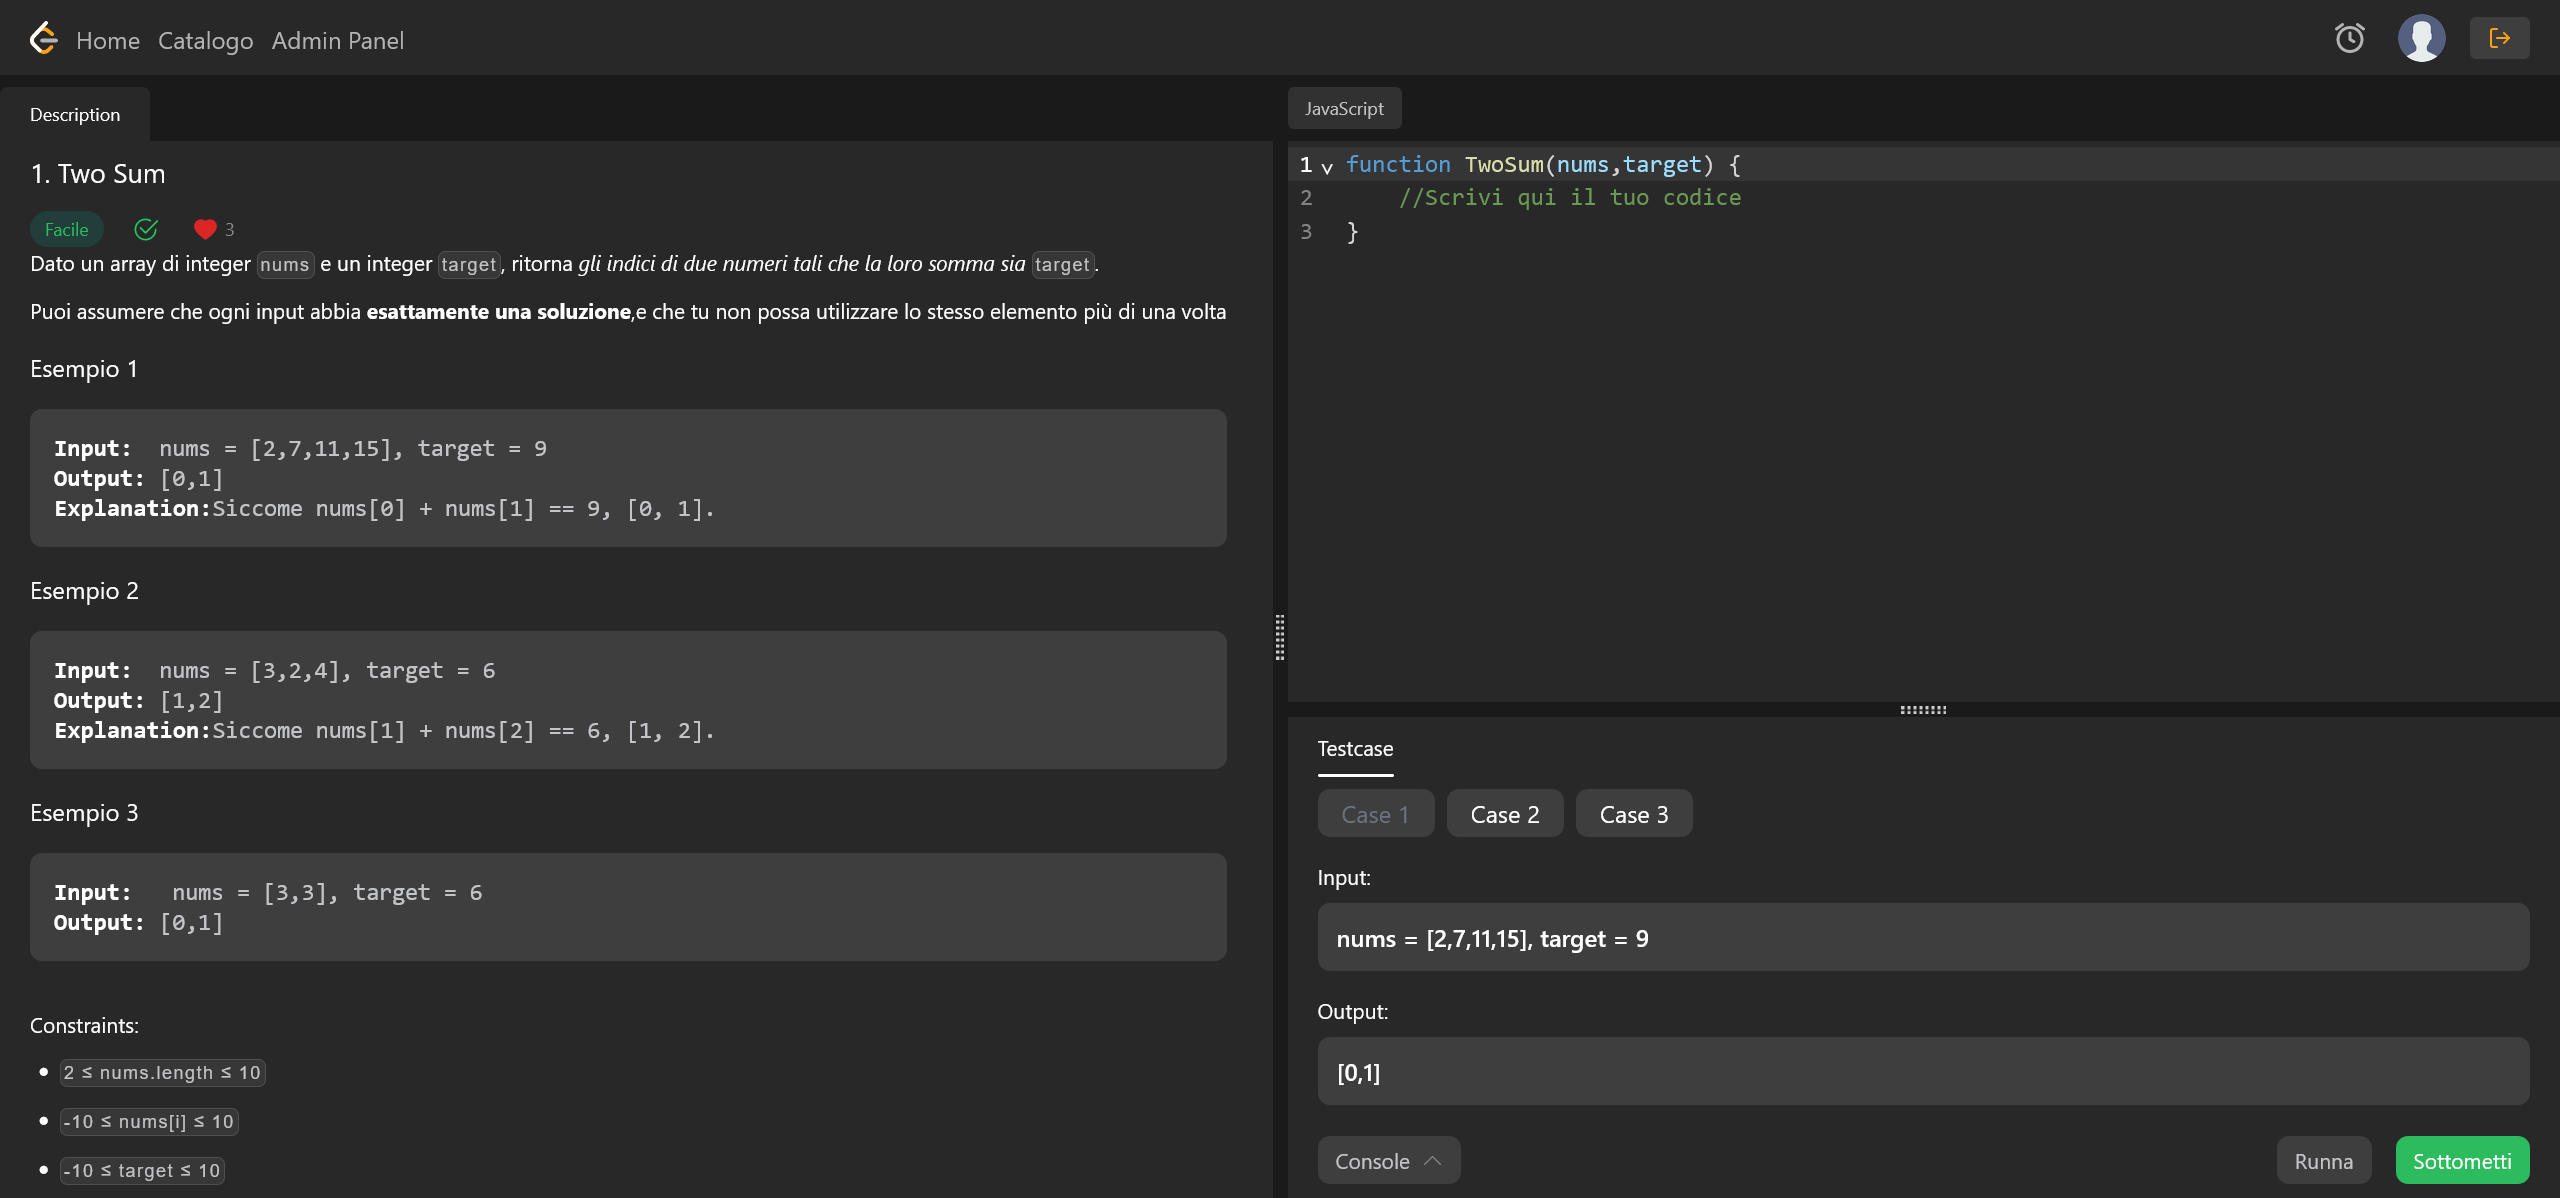
\includegraphics[width=\textwidth]{materiale/sito/Problema.png}

\newpage
\section{Github Repository e Deployment Info}
La repository del progetto è disponibile al seguente link:
\begin{center}
  \href{https://github.com/G17-UniTn}{G17-UniTn}
\end{center}
La repository è suddivisa in 3 parti:
\begin{itemize}
  \item "Deliverables" contentente tutti i PDF e le immagini dei deliverables assieme ai file .tex
  \item "Documents" contentente tutti i PDF e solo i PDF.
  \item "CodeBase" contiene tutto il codice relativo al FrontEnd ed al BackEnd.
\end{itemize}Il gruppo che ha sviluppato il progetto è composto dai seguenti membri:
\begin{itemize}
  \item Raffaele Castagna \href{https://github.com/Raffaele-Castagna}{\faGithub}
  \item Zeno Saletti \href{https://github.com/zenosalty}{\faGithub}
  \item Alberto Rovesti \href{https://github.com/uniBeto}{\faGithub}
\end{itemize}Il sito è attualmente attivo ed hostato sulla piattaforma vercel, di seguito riportiamo il link per visualizzare la pagina web.
\begin{center}
  \url{https://sleepcode-dev.vercel.app/}
\end{center}
Per poter testare il sito abbiamo creato un account che ha i privilegi di amministratore:

\begin{itemize}
  \item Email: "admin@gmail.com", password: "PasswordAdmin2024!"
\end{itemize}
Ricordiamo che pultroppo non siamo stati in grado di dare tutte le funzionalità descritte nel D2 all'amministratore, tuttavia il pannello accessibile solo ad utenti amministratore è funzionante.\\\\
Ricordiamo anche che il processo di invio email per recupero password e la pagina dove immettere la nuova password è gestito da terze parti, e le regole per la password non possono essere utilizzate se si richiede un recupero password.
\newpage
\section{Testing}
Per eseguire il testi abbiamo utilizzato il pacchetto \href{https://jestjs.io/}{Jest} e l'abbiamo integrato con Firebase con il pacchetto \href{https://www.npmjs.com/package/firestore-jest-mock}{Jest-firestore-mock}, per simulare le richieste API abbiamo
utilizzato il pacchetti \href{https://www.npmjs.com/package/node-mocks-http}{node-mocks-http}.\\
Abbiamo definito 2 cartelle "\href{https://github.com/G17-UniTn/CodeBase/tree/master/__mocks__}{\_\_mocks\_\_} e \href{https://github.com/G17-UniTn/CodeBase/tree/master/__test__}{\_\_test\_\_}, la prima è stata creata per utilizzare le funzioni di "mock" di jest 
che permettono a jest di "imitare" connessioni al database e/o credenziali, molto utile nel testing di API che richiedevano funzioni disponibili solo alla \href{https://firebase.google.com/docs/reference/admin}{SDK admin} di firebase
\\\\
Di seguito riportiamo le diverse test suite create\\\\
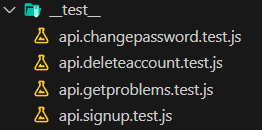
\includegraphics[width=\textwidth]{materiale/testing/test-overview.png}
\subsection{Test API}
Di seguito sono mostrati i risultati delle test suite applicate sulle diverse API
\subsubsection{test api/signup}
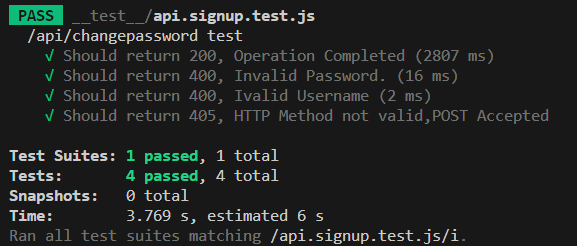
\includegraphics[width=\textwidth]{materiale/testing/Signup.png}
\subsubsection{test api/changepassword}
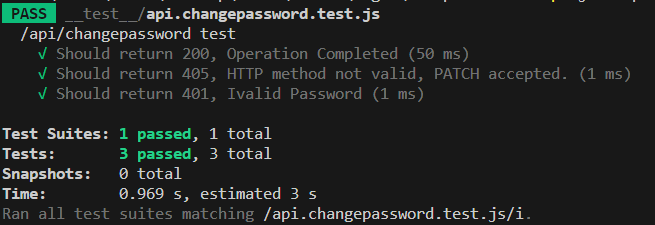
\includegraphics[width=\textwidth]{materiale/testing/ChangePw.png}
\subsubsection{test api/deleteAccount}
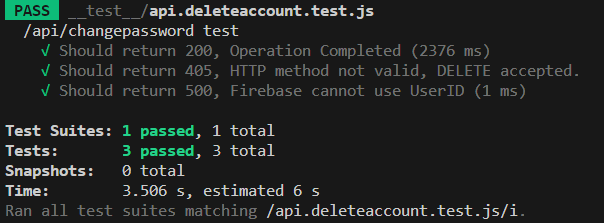
\includegraphics[width=\textwidth]{materiale/testing/DeleteAccount.png}
\subsubsection{test api/getProblems}
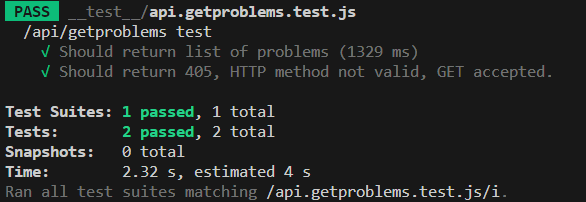
\includegraphics[width=\textwidth]{materiale/testing/GetProblems.png}
\newpage
\subsection{Code Coverage}
Di seguito riportiamo il code coverage generato da JEST.\\\\
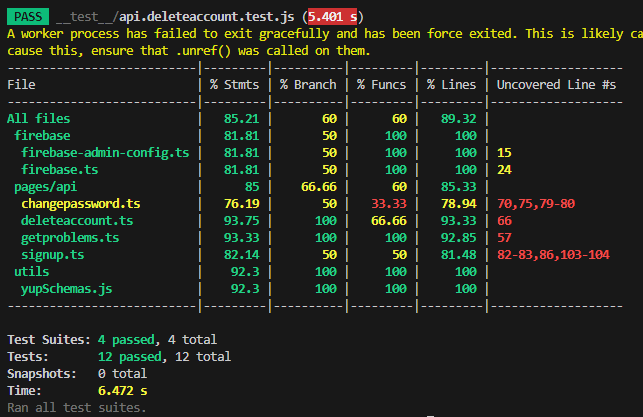
\includegraphics[width=\textwidth]{materiale/testing/Code Coverage.png}
\end{document}